\documentclass[11pt, a4, nocenter, margin=150mm]{article}

\usepackage[top=20mm, bottom=20mm, inner=25mm, outer=25mm]{geometry}
\usepackage[title, toc]{appendix}
\usepackage{array}
\usepackage[font=scriptsize, labelfont=it, textfont=it]{caption}
\usepackage{graphicx}
\usepackage{setspace}
\usepackage{enumitem}
\usepackage[parfill]{parskip}
\usepackage{multirow}

\newcolumntype{A}{>{\centering\arraybackslash}m{0.9cm}}
\newcolumntype{B}{>{\centering\arraybackslash}m{1.3cm}}
\newcolumntype{C}{>{\centering\arraybackslash}m{1.5cm}}
\newcolumntype{D}{>{\centering\arraybackslash}m{1.8cm}}
\newcolumntype{E}{>{\centering\arraybackslash}m{2cm}}
\newcolumntype{F}{>{\centering\arraybackslash}m{4.2cm}}
\newcolumntype{G}{>{\centering\arraybackslash}m{5.4cm}}
\setlength{\parindent}{0pt}

\begin{document}

%%%%%%%%%%%%%%%%%%%%%%%%%%%%%%%%%%%%%%%%%%%%%%%%%%%%%%%%%%%%%%%%%%%%%%%%%%%%%%%%
\onehalfspacing
\begin{titlepage}
	\begin{center}
		\Huge
		\textbf{UNSW} \\

		\vspace{5mm}

		
\includegraphics[height=4cm]{unsw-logo.jpg}

		\vspace{5mm}

		\Large
		Faculty of Engineering \\
		School of Mechanical \& Manufacturing Engineering \\

		\vspace{10mm}

		\textbf{MMAN3000} \\
		Professional Engineering \& Communication \\

		\vspace{15mm}

		\LARGE
		\textbf{Individual Report Assessment} \\
		F13-SG-Group2

		\vspace{15mm}

		\Large
		Course Coordinator: Zoran Vulovic\\
		Due Date: 18/08/2020 \\

		\vfill
		\rule{\linewidth}{0.5pt} \\

		\Large
		Dan Nguyen \\

		\large
		z5206032 \\

	\end{center}
\end{titlepage}

%%%%%%%%%%%%%%%%%%%%%%%%%%%%%%%%%%%%%%%%%%%%%%%%%%%%%%%%%%%%%%%%%%%%%%%%%%%%%%%%
\pagenumbering{roman}
\tableofcontents
\vspace{1cm}
\listoffigures
\vspace{1cm}
\listoftables
\pagebreak

\pagenumbering{arabic}

%%%%%%%%%%%%%%%%%%%%%%%%%%%%%%%%%%%%%%%%%%%%%%%%%%%%%%%%%%%%%%%%%%%%%%%%%%%%%%%%
\section{Individual Work}

	My MMAN3000 workflow centred around Microsoft Office Powerpoint due to its powerful diagram and shape tools which allowed me to draft and present ideas quickly. All the work done have been screenshotted and included in the appendices as visualisation of the work but will be discussed in this section. The individual work is outlined in a weekly timeline in Figure \ref{fig:timeline} below.

	\begin{figure}[h!]
		\centering
		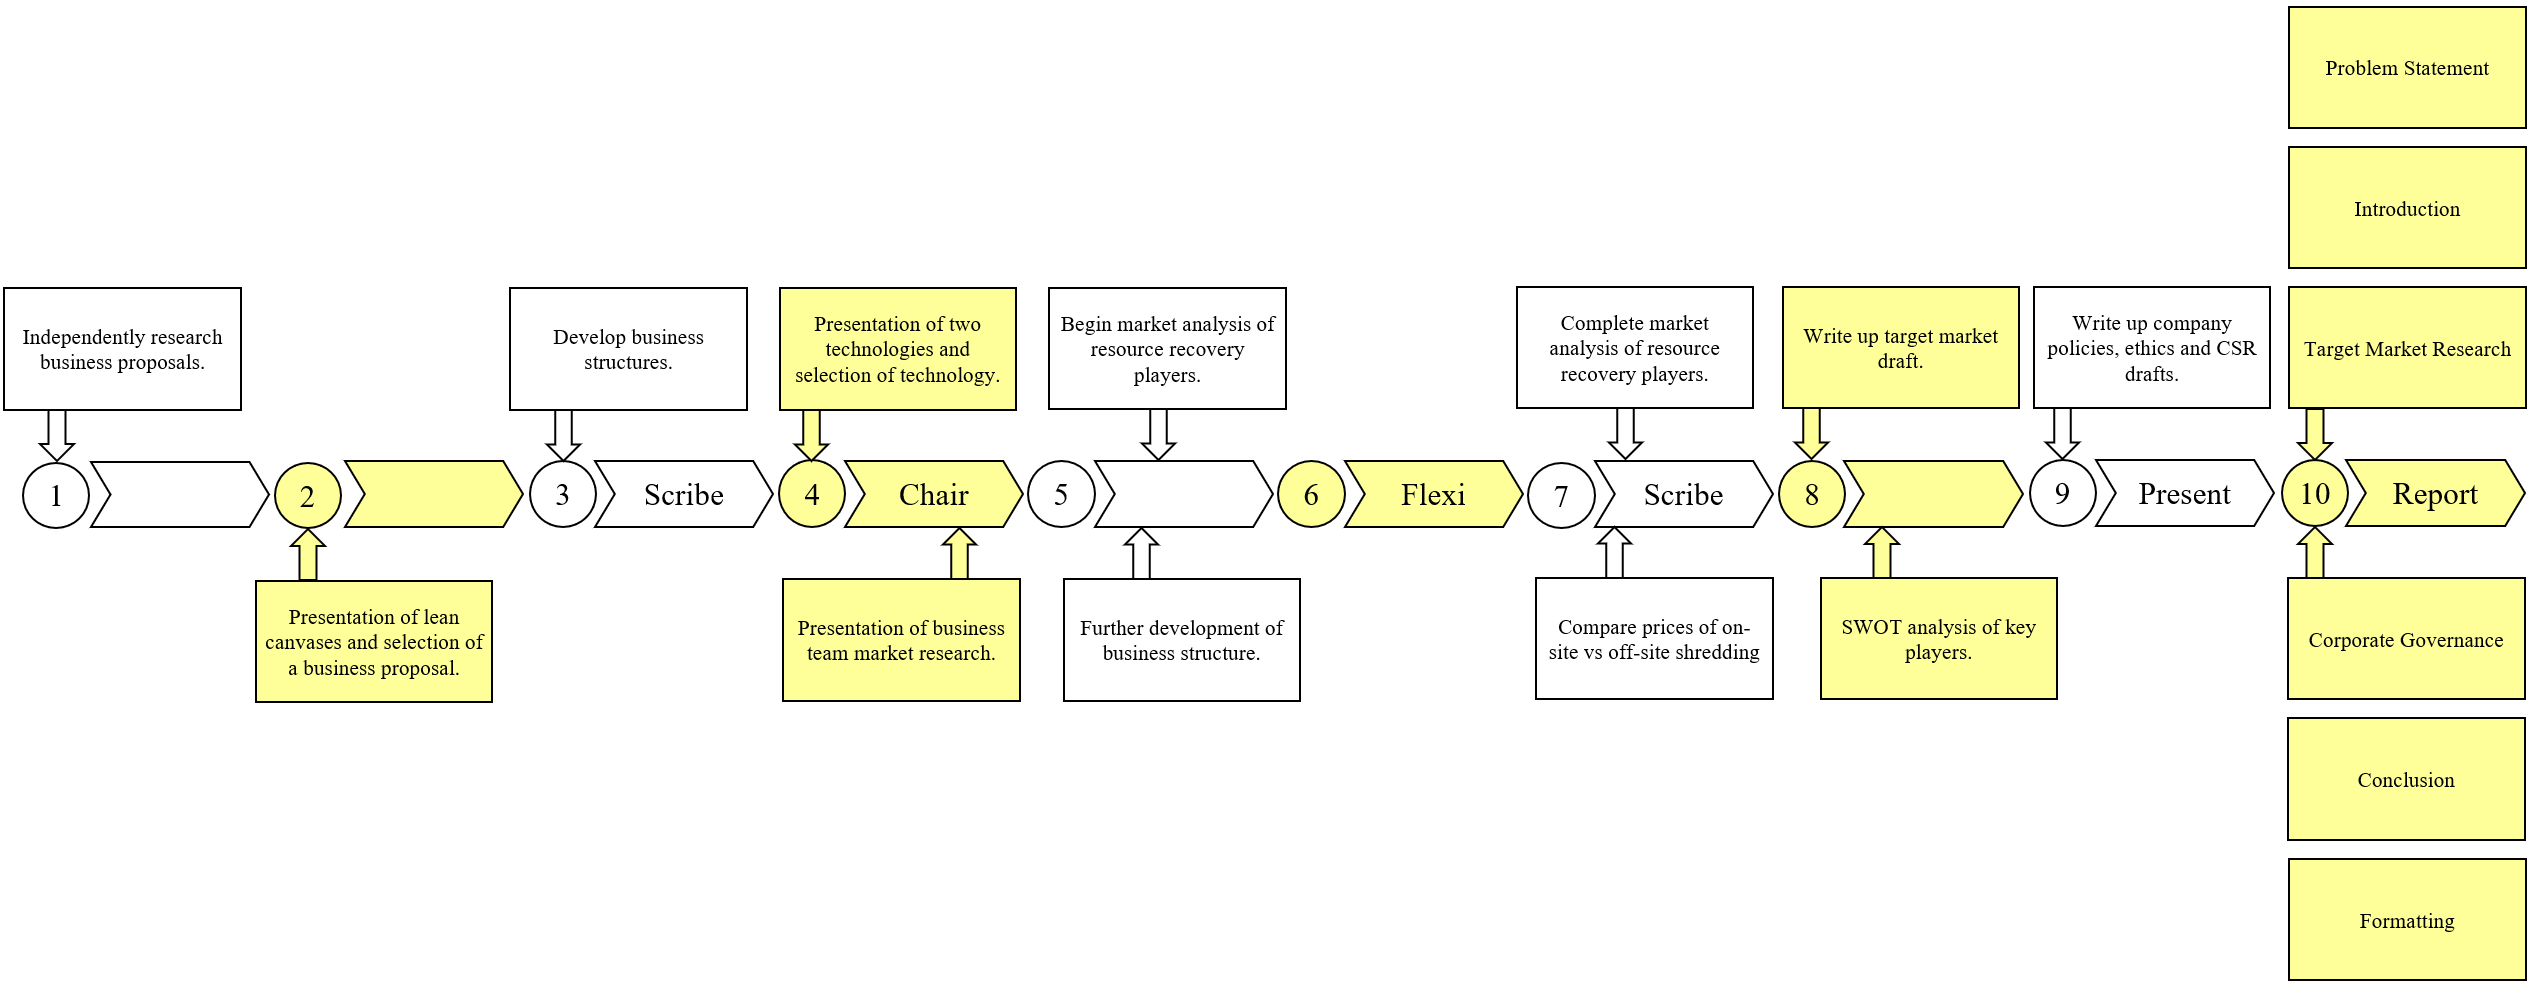
\includegraphics[width=\textwidth]{timeline.png}
		\caption{Weekly Timeline of Tasks}
		\label{fig:timeline}
	\end{figure}

	\subsection{Week 1}

	The first team meeting tasked everyone with individual research into a potential business idea. I first proposed a business in designing, manufacturing and retailing firefighting UGVs to firefighting services, organisations or individuals in response to the recent 2020 Australian bushfires where manpower was lacking and would require firefighters to put their lives in direct danger. My second business proposal is a machining workshop which would provide a service to machining students, engineers, and hobbyists for access to machining tools (e.g. lathe, mill). This solves the customer's difficulty in access to such machines, lack of money to purchase the machines, or non-suitable environment to house the machines.

	These business proposals were formatted onto lean canvases (see Appendix \ref{app:lean_canvas}) which covered the important aspects to consider for starting up a business i.e. problem statement, solution, key metrics, unique value proposition, advantages in the market, public relationship channels, customer segments, cost structure and revenue streams.

	\subsection{Week 2}

	The two business proposals were presented on the Monday of week two and were well-received.

	The week two meeting assigned everyone with the task of developing a business structure for the group's selected business proposal i.e. Michael's automated recycling. I proposed several business structures (proprietary, public, start-up) as the operations of the business had not been finalised (see Appendix \ref{app:business_structures}). I had also included an exploded business structure which described job responsibilities.

	\subsection{Week 3}

	I had the responsibility of scribing for week 3 (see Appendix \ref{app:week3_scribe}).
	
	As required from the week 2 meeting, I have researched into business structures and responsibilities to cover various operations of the business (see Appendix \ref{app:business_structures}). There was difficulty however in finalising the business structure as the business operations had not been finalised. Therefore I developed multiple potential business structures (e.g. proprietary, public, start-up).

	\subsection{Week 4}

	I had the responsibility for chairing for week 4 for which I planned and uploaded agendas for two meetings (see Appendix \ref{app:week4_chair}). The first (Monday) meeting agenda required each person to present two technologies. In the agenda, I outlined the problem statement, market summary from the previous meeting, and potential questions to answer in aiding the technology research. I also planned the course of action for discussion of technologies and listed expected outcomes for the end of the meeting.

	My own presentation of the two technologies focused on the kerbside recycling phase of the plastic waste cycle (see Appendix \ref{app:technology_research}) - ensuring waste is properly sorted before it is collected. These technologies were: BinBot!, an automated rubbish sorter; and Bin Buddy, a phone app which scans rubbish and highlights the kerbside bin the rubbish belongs in. I presented the technologies with the general designs, processes, and estimated cost.

	A challenge arose however where each proposed technology solved a different problem (tackled different aspects of the waste lifecycle). The challenge and its resolution will be outlined in Table \ref{tab:challenges} in Section \ref{sec:project}.

	I prepared a second agenda for the next (Friday) meeting which included each team's objectives for the week, action plan for the meeting and expected outcomes.

	My contribution for the business team involved the waste management and resource recovery market research (Appendix \ref{app:market_research}). These two markets can be subcategorised by type of material where I did further research into the paper \& cardboard, glass, plastics, and rubber market. With each of these markets, I included market trends, future/current events affecting the market, stakeholders, competitors, and resources used.

	At the end of the Friday meeting, I strongly pushed for the selection of a technology as delaying the selection would have timely consequences.

	\subsection{Week 5}

	Began market share research into resource recovery players.

	\subsection{Week 6}

	No work.

	\subsection{Week 7}

	I scribed for week 7 meetings in Michael's absence (Appendix \ref{app:week7_scribe}).

	I took up the task of comparing on-site verse off-site shredding prices (Appendix \ref{app:shred}). Research for off-site plastic shredders was difficult as there is no demand for such services and do not list their prices without consulting. I calculated the initial cost from a gross market value from cheap to expensive shredders and calculated the operational cost for a gross electricity bill and labour wages.

	I completed the market share analysis into major resource recovery players (Appendix \ref{app:market_share}). The market value of proprietary companies is difficult to obtain. Therefore, their estimate revenue value is obtained to correlate the company size. A pie graph was created to visualise this information. Other information obtained was the amount of plastic processed per year, types of waste plastic accepted, and types of plastic manufactured.

	\subsection{Week 8}

	Drafted up target market research for the report. The draft included the target market, stakeholders, direct competitors, waste levy, and waste export bans (see Figure \ref{fig:draft} in Appendix \ref{app:draft}).

	A SWOT analysis of competitors was also completed for the largest and relevant players from the target market such as Visy, Replas, and Licella (see Appendix \ref{app:swot}). SWOT is an acronym for strengths, weaknesses, opportunities, threats - where strengths and weaknesses are internal attributes, and opportunities and threats are external influences. This analysis is methodical for identifying opportunities for our company and raises awareness of strengths and weaknesses inherent to the market \cite{swot}.

	\subsection{Week 9}

	Drafted up ethics, corporate governance, and company policies for the report and presentation (see Figure \ref{fig:ethics} in Appendix \ref{app:draft}).

	\subsection{Week 10}

	My contribution to the final report covered writing up the problem statement, introduction, parts of the target market research, corporate governance, some contribution to ethics, conclusion, editing and formatting the report (Figure \ref{fig:report1} of Appendix \ref{app:final}). Yellow highlights in the figures in Appendix \ref{app:final} are my own words, and green highlights are contributions to other people's works.

	In target market research section (Figure \ref{fig:report1} of Appendix \ref{app:final}), I provided a tabulated summary (Table 1 from the Final Report \cite{report}) for ease of understanding of the context of the crude oil and waste management markets that Aww Mman were participating in. This table included risks, opportunities, relevant stakeholders, and competitors. The target market research section was outlined like so: crude oil and waste management. With each of these markets discussed in detail with respect to its opportunities. The section was discussed with statistics and referencing to fully justify Aww Mman's position and interests in the market.

	As a side note, no research had been performed on the crude oil market throughout the term. Therefore, Jeff laid out some research in the report but I expanded on the work with further correct research, referencing and analysis of the trends of the market.

	I wrote the competitor analysis section (Figure \ref{fig:report1} of Appendix \ref{app:final}), however only one company was included from the SWOT analysis i.e. Licella. This is due to the lack of direct competitiveness of Visy and Replas, and difficulty of performing SWOT analyses on more players due to lack of free information. Direct competitors in the crude oil market were not named due to the large number of global players, it was not worth performing a SWOT analysis on key players.

	I wrote the corporate governance section of the report (Figure \ref{fig:report2} of Appendix \ref{app:final}) to justify the workforce structure, as well as how corporate governance will influence the operations of the business through a summary of a subset of corporate policies in Table 3 of the Final Report \cite{report}.

	My more minor contributions (Figure \ref{fig:report3} of Appendix \ref{app:final}) is passing the drafted work on ethics and CSR to the final report which Lucy expanded on. I had written up most of the conclusion to summarise each section of the report. I provided a skeleton for the technology paragraph in the conclusion for which Neil wrote.

	My contributions for the report are supported by the compilation of waste levy rates in Appendix A of the Final Report \cite{report}, analysis of produced vs imported crude oil trends in Appendix B of the Final Report \cite{report}, SWOT analysis of Licella in Appendix D of the Final Report \cite{report}, and summary of company policies in Appendix G of the Final Report \cite{report}. These contributions are in Figures \ref{fig:report4} and \ref{fig:report5} of Appendix \ref{app:final}.

	Further contributions are editing and formatting the report where I:
	
	\begin{itemize}[noitemsep, nolistsep]
		\item standardised the spelling of words (e.g. bio-fuel and biocrude);
		\item standardised the use of mathematical symbols, numbers, and units;
		\item corrected grammar;
		\item enforced consistent referencing;
		\item removed of non-informative text;
		\item formatted page numbering for roman numerals before the introduction and arabic numerals afterwards;
		\item cleaned up IEEE references to be neat and correct; and
		\item cleaned up appendices to be neat.
	\end{itemize}

%%%%%%%%%%%%%%%%%%%%%%%%%%%%%%%%%%%%%%%%%%%%%%%%%%%%%%%%%%%%%%%%%%%%%%%%%%%%%%%%
\section{Project Evaluation}
\label{sec:project}

	\subsection{Challenges}

	There were numerous challenges that arose as a result of the action plan the team had taken early in the project. The challenges and the team's resolutions are tabulated in Table \ref{tab:challenges}.

	\begin{table}[h!]
		\footnotesize
		\centering
		\caption{Project Challenges}
		\label{tab:challenges}
		\begin{tabular}{|C|G|C|G|}
			\hline
			\textbf{Date} & \textbf{Challenge} & \textbf{Date} & \textbf{Resolution} \\
			\hline
			Friday, Week 2 & Incorrect use of lean canvases lead to selection of business proposal that was not fully defined. & - & This challenge was not identified. \\
			\hline
			Monday, Week 3 & Non-confirmation of problem statement misguided market research. & - & This challenge was not identified. \\
			\hline
			Friday, Week 3 & Business structures could not be finalised as technology had not been selected. & Monday, Week 4 & Research and present two technologies for selection before progression. \\
			\hline
			\multirow{5}{1.5cm}{\centering Monday, Week 4} & \multirow{5}{5.4cm}{\centering Proposed technologies did not solve a common problem statement or tackled the same market.} & Monday, Week 4 & Defined the waste lifecycle, selected a more specific market, confirmation of problem statement and narrowed list of technologies for further evaluation. \\
			\cline{3-4}
			& & Friday, Week 4 & Splitting the group into technology team to research viability of narrowed technologies and business team to research profitability of markets in waste lifecycle. \\
			\hline
			Monday, Week 5 & Lack of chairing responsibility led to uncertainty in week 5 and snowballed with the loss in seriousness of the responsibility. & - & This challenge was not addressed. \\
			\hline
	    \end{tabular}
	\end{table}

	There was also no team conflicts.

	\subsection{Redoing the Project}

	If I redid the MMAN3000 business proposal assignment, I would suggest each person in the team to present their business proposals in lean canvases in week 1. However, these lean canvases must be filled out properly with clear problem statements and a list of proposed solutions. Therefore, it is best to set expectations by providing an example lean canvas to the team.
	
	The lean canvases when filled out will create a skeleton for the business model where a technology team and operations team can flesh out the categories of the lean canvas in detail. The new set of weekly deliverables are in Table \ref{tab:deliverables} below.

	\begin{table}[h!]
		\footnotesize
		\centering
		\caption{Deliverables}
		\label{tab:deliverables}
		\begin{tabular}{|c|F|F|F|}
			\hline
			\textbf{Week} & \textbf{General} & \textbf{Technology} & \textbf{Operations} \\
			\hline
			1 & - & - & - \\
			\hline
			2 & Lean canvases \& problem statement & Technology research & Target market research \\
			\hline
			3 & Technology selection & System overview & Marketing strategy \\
			\hline
			4 & - & Component research & Revenue streams \\
			\hline
			5 & - & Component research & Workforce structure \\
			\hline
			6 & - & Component research & Cost structure \\
			\hline
			7 & - & Plant setup & Regulations \\
			\hline
			8 & - & Australian standards & Business ethics \\
			\hline
			9 & Presentation & - & - \\
			\hline
			10 & Report & - & - \\
			\hline
	    \end{tabular}
	\end{table}

	General deliverables requires work from both technology and operations teams. Each member will contribute lean canvases, finalise the problem statement, select a technology, and work on the presentation and report.

	The order of deliverables for the technology team is technology research, technology selection (with input from operations team), system overview, component research, plant setup, and Australian standards. All purchases and workforce requirements need to be communicated to the operations team to account for the workforce and cost structure. The order of deliverables for the operations team is target market research, marketing strategy, revenue streams, workforce structure, cost structure, regulations, and business ethics.

%%%%%%%%%%%%%%%%%%%%%%%%%%%%%%%%%%%%%%%%%%%%%%%%%%%%%%%%%%%%%%%%%%%%%%%%%%%%%%%%
\section{Team Evaluation}

	In a general evaluation, this group is so far the best group I have been in for an academic assignment. It is a group of highly motivated people with histories of excellence in academia and extra-curricular activities. An evaluation for each member including myself will be based off the marking criteria in Appendix \ref{app:marking_criteria}. The appendix will have details to the distribution and justification of marks.

	For my rationale on the marking criteria, there is a total of twenty marks which is accumulated from each criterion. The amount of contribution and quality of contribution each have a five marks where each mark is given on a qualitative assessment. I have assigned a mark of three for chairing responsibility and two for scribing responsibility - where I consider chairing more important. This is because (from my understanding) the course had a strong expectation of sharing the chairing and scribing responsibility each week, so that each member of the team had a chance to prove their administration skills. Morale has two marks, which covered the team member's impressions. Discussion has three marks, which covers the team member's initiative to participate in team discussion.

	Table \ref{tab:scores} outlines the scores for each criterion for each team member.

	\begin{table}[h!]
		\scriptsize
		\centering
		\caption{Team Member Evaluation Scores}
		\label{tab:scores}
		\begin{tabular}{CCCBBCEC}
			\hline
			\hline
			\multirow{2}{1.5cm}{\centering \textbf{Team Member}} & \textbf{Amount} & \textbf{Quality} & \textbf{Chair} & \textbf{Scribe} & \textbf{Morale} & \textbf{{Discussion}} & \textbf{Overall} \\
			& (5 marks) & (5 marks) & (3 marks) & (2 marks) & (2 marks) & (3 marks) & (20 marks) \\
			\hline
			\hline
			Lucy & 5 & 5 & 3 & 0 & 2 & 3 & 18 \\
			\hline
			Dunya & 5 & 5 & 3 & 2 & 2 & 3 & 20 \\
			\hline
			Michael & 5 & 4 & 0 & 2 & 2 & 2 & 15 \\
			\hline
			Neil & 4 & 4 & 2 & 2 & 1 & 2 & 15 \\
			\hline
			Jeff & 3 & 3 & 2 & 2 & 2 & 2 & 14 \\
			\hline
			Felix & 1 & 2 & 0 & 1 & 0 & 0 & 4 \\
			\hline
			Arfin & 5 & 5 & 3 & 0 & 2 & 3 & 18 \\
			\hline
			Dan & 4 & 3 & 3 & 2 & 1 & 2 & 15 \\
			\hline
	    \end{tabular}
	\end{table}

	\subsection{Lucy Birdsey}

	Lucy started off the term very strongly as chairperson, with uploaded agenda for week 2, and clear organisation and direction of meetings. Lucy also organised the week 6 meetings. Lucy earned three marks for chairing responsibility. Unfortunately, Lucy did not get a chance to scribe (or I could not find the relevant minutes). Therefore earning zero marks for scribing responsibility.

	Lucy's contribution covered aspects of technology (for which I do not have full knowledge of), and presentation and report writing of ethics \& CSR. The amount of work put into the presentation and report writing which I saw was of excellent quality and required no editing or revision. Therefore, earning a mark of five for both amount and quality of contributions.

	Lucy is very empathetic and often shows appreciation of the work and effort people put in which consequently boosts team morale. Therefore, Lucy earned two marks for morale. She is also extremely active in discussions (e.g. suggesting an ideal situation in the problem statement of the Final Report \cite{report} and proposing the research of two technologies when the business structures challenge arose) and will attempt to open dialogue when there is a pause in discussions. Therefore, Lucy earned three marks for discussion.

	\subsection{Dunya Vasic}

	I found Dunya to be the strongest character in the team. She is extremely driven which is best demonstrated when she tried to contact Licella and various resource recovery companies to obtain information to support her technical findings. She succeeded in organising a meeting with a Licella employee. Dunya had written the majority of the technology section in the report to very good quality with minimal edits. I believe Dunya is deserving of five marks for amount and quality of contribution.

	Despite the fallout of chairing responsibility in week 5. Dunya maintained her responsibility with the uploading of agendas and management of meetings in week 7. Dunya also scribed in week 6 of good quality. Therefore, Dunya earned three marks for chairing and two marks for scribing.

	Dunya had high enthusiasm, actively participated in team discussions and quick to critically analyse topics in discussion. She also consistently encouraged communication (e.g. expressing concern when not enough dialogue was opened). Therefore, Dunya earned two marks for morale and three marks for discussion.

	\subsection{Michael Currie}

	Michael has contributed a lot of work into the research and write up of regulations for the final report as well as technology work through the term. His work required minimal revision as I had to edit some of the regulations to make it more relevant to Aww Mman's operations. Therefore, Michael receives a mark of five for the amount and mark of four for the quality of contribution.

	Unfortunately, I could not find meetings that Michael had facilitated therefore, giving him a mark of zero for chairing responsibility. Michael had initiative to accept scribing responsibility for Monday Week 4 (in Felix' absence) but was unfortunately unavailable to scribe in his specified week due to unforeseen circumstances. Therefore, Michael receives an adjusted mark of two for scribing.

	Michael was enthusiastic and always had his camera on (despite being the only person in the team to do so). He had moderate participation in discussion as he became noticeably less active in the latter half of the term. Therefore he received a mark of two for moral and two for discussion.
	
	\subsection{Neil Yang}

	Neil is reliable in that he completes the tasks that he is assigned. The quality of his work is also very good, requiring no need for revision. Therefore, he received a mark of four for both amount and quality of contribution.

	Neil uploaded agenda and had clear goals for meetings (week 9). Neil had excellent initiative taking up scribe responsibility for weeks 6, 8, and 9 meetings. Therefore, receiving a mark of two for both responsibilities.
	
	Neil does not have a strong active voice, but knows when to raise his voice. As such, he displayed moderate enthusiasm and moderate participation to discussion - earning him one mark for morale and two marks for discussion.

	\subsection{Jeff Chang}

	Jeff completed most of his tasks. The task that he did not complete was the business market research of week 3 and the business structure was completed too late (completed at time of report writing). The quality of contribution was good but required me to edit to add more detail or reword for easier understanding (e.g. in the crude oil market section of the Final Report \cite{report}). This justifies Jeff's mark of three for both amount and quality of contribution.
	
	Jeff had some organisation in his chairing responsibility in week 3. He had a late upload of the agenda and tried to take charge of the meeting when dialogue had died. Jeff was on top of his scribing responsibility, delivering concise minutes for week 2 and offered to scribe for Friday week (covering for Felix). Therefore, Jeff earned a mark of two for both chairing and scribing.

	Jeff is easy to socialise with but did not provide strong enthusiasm for the project. Therefore, earning a mark of two marks for morale.
	
	Jeff had moderately participated to discussions whether it be asking a question for assurance or providing an opinion on a topic. Jeff earned a mark of two for the discussion.

	\subsection{Hao Jin (Felix)}

	Felix had poor, irregular attendance for which I had to email and message him to ensure his attendance. His absence had no impact on team morale and did not allow him to participate in discussions. Therefore, Felix receives a zero mark for morale and discussion.

	Felix had the responsibility to scribe for week 4 however was only present to scribe for the Friday meeting. He also scribed the Friday week 4 meeting but incorrectly identified me as facilitator. With the scribe responsibility partially fulfilled, Felix earns a mark of one.

	Felix had the responsibility to chair for week 5. He uploaded an agenda for the Friday meeting and was present but did not communicate at all during the meeting therefore failing to act as chairperson. For this, Felix received a mark of zero.

	I am unaware of Felix contributing any work throughout the term. His only contribution is in the final report, therefore earning him a mark of one for the amount of contribution for minimal effort.

	During my review of the final report, Felix had made references to wikipedia and YouTube. I had to research the topics and change the references to more reliable sources to ensure the quality of the report was not compromised. This poor quality of referencing makes me question the quality of his report work (in its authenticity). Reviewing his written section of the report, it contained some relevant information and a concise table of technologies. Therefore, Felix' work is limited to a fair quality grade, giving him a mark of two for quality of contribution.

	Some unusual behaviour from Felix was discovered upon my comparison between new and old versions of my team's minutes. Felix had added his name to the present list (when absent) to week 2 official and week 7 official minutes after they had been uploaded to Teams.

	\subsection{Muhammad Arfin}

	Arfin has excellent initiative and contributed a large amount of work into the project overall, mainly business and operations. Arfin produced excellent quality work with great attention to detail. His work required no revision or editing. Therefore, he earned a mark of five for both amount and quality of contribution.

	Unfortunately, I am not aware of Arfin having taken chairing and scribing responsibility (as I could not find the minutes). However, he has proven his administration skill through the organisation of splitting the team into subteams of technology and business, and the responsibilities of each subteam. Arfin had also written a sequence of tasks for the business team to complete which showed his holistic understanding of business operations. Therefore, I gave Arfin an adjusted chairing mark of three and scribing mark of zero.

	Arfin had high enthusiasm and encouraged the early completion of the project. He has good social impressions and was very active in discussions especially concerning business and operations. Therefore, Arfin received a mark of two for morale and three for discussion.

	\subsection{Dan Nguyen}

	The amount and quality of contribution I had put in was decent. In the business work, I often felt stuck, in that I did not know what I was doing as I had no guidance or good resources. This is best demonstrated in the market share analysis work which took me two weeks to complete as most information about competitors and the market had to be bought. Therefore, I had to complete the market analysis using the company's revenue value to correlate the business size and therefore its market value. This revenue value is thanks to various news media sources and ZoomInfo \cite{zoom}. The notion of purchasing information is also true for SWOT analyses, where it was difficult to obtain sensitive information about companies - I wish I could explore more competitors in the final report. I felt as though the introduction that I had written for the final report was lacking in showing the framework of the report. My quality of work can shine e.g. in the Licella SWOT analysis (Figure \ref{fig:report1}), corporate governance write-up (Figure \ref{fig:report2}), crude oil market research (Figures \ref{fig:report1} and \ref{fig:report4}), and company policy write-up \ref{fig:report5}. I felt as though my work here is highly justified and supported by thorough research and analysis. Therefore, I feel four marks for amount of contribution and three marks for quality of contribution is justified.

	In my chairing responsibility, I thoroughly organised my agendas and uploaded them with haste. I also tried my best to take charge of meetings and come to conclusions. I was on top of my scribing responsibility, ensuring, I did not miss any information and asking questions in case I did. I uploaded these minutes immediately after the conclusion of the meetings. Therefore, I feel three marks for chairing and two marks for scribing is justified.

	I showed moderate enthusiasm and moderate participation to team discussion. The times when my participation had dropped are during meetings which were technology-heavy, as I had no opinions as my work was focused on business. My showcase of enthusiasm may not be very high because I felt as though my team already had too many highly enthusiastic people (it is difficult to stand-out especially online). I believe I would have no trouble with participation, if meetings were done in person. I feel that one mark for morale and two marks for discussion is justified.

\pagebreak

%%%%%%%%%%%%%%%%%%%%%%%%%%%%%%%%%%%%%%%%%%%%%%%%%%%%%%%%%%%%%%%%%%%%%%%%%%%%%%%%
\begin{thebibliography}{3}

	\bibitem{report} M. Arfin, et al., "Team Project Report," UNSW, School of Mechanical \& Manufacturing Engineering, Aug. 2020.

	\bibitem{swot} C. White, \emph{What's a Competitive Analysis \& How Do You Conduct One?}, Nov, 13, 2019. https://blog.hubspot.com/marketing/competitive-analysis-kit.

	\bibitem{zoom} ZoomInfo. Accessed on: Nov. 17, 2020. [Online]. Available: https://www.zoominfo.com/.

\end{thebibliography}

\pagebreak

%%%%%%%%%%%%%%%%%%%%%%%%%%%%%%%%%%%%%%%%%%%%%%%%%%%%%%%%%%%%%%%%%%%%%%%%%%%%%%%%
\begin{appendices}

\section{Lean Canvas}
\label{app:lean_canvas}
	
	Lean canvas business proposals for firefighting UGV (Figure \ref{fig:ugv_lean_canvas}) and machining workshop (Figure \ref{fig:workshop_lean_canvas}).

	\begin{figure}[h!]
		\centering
		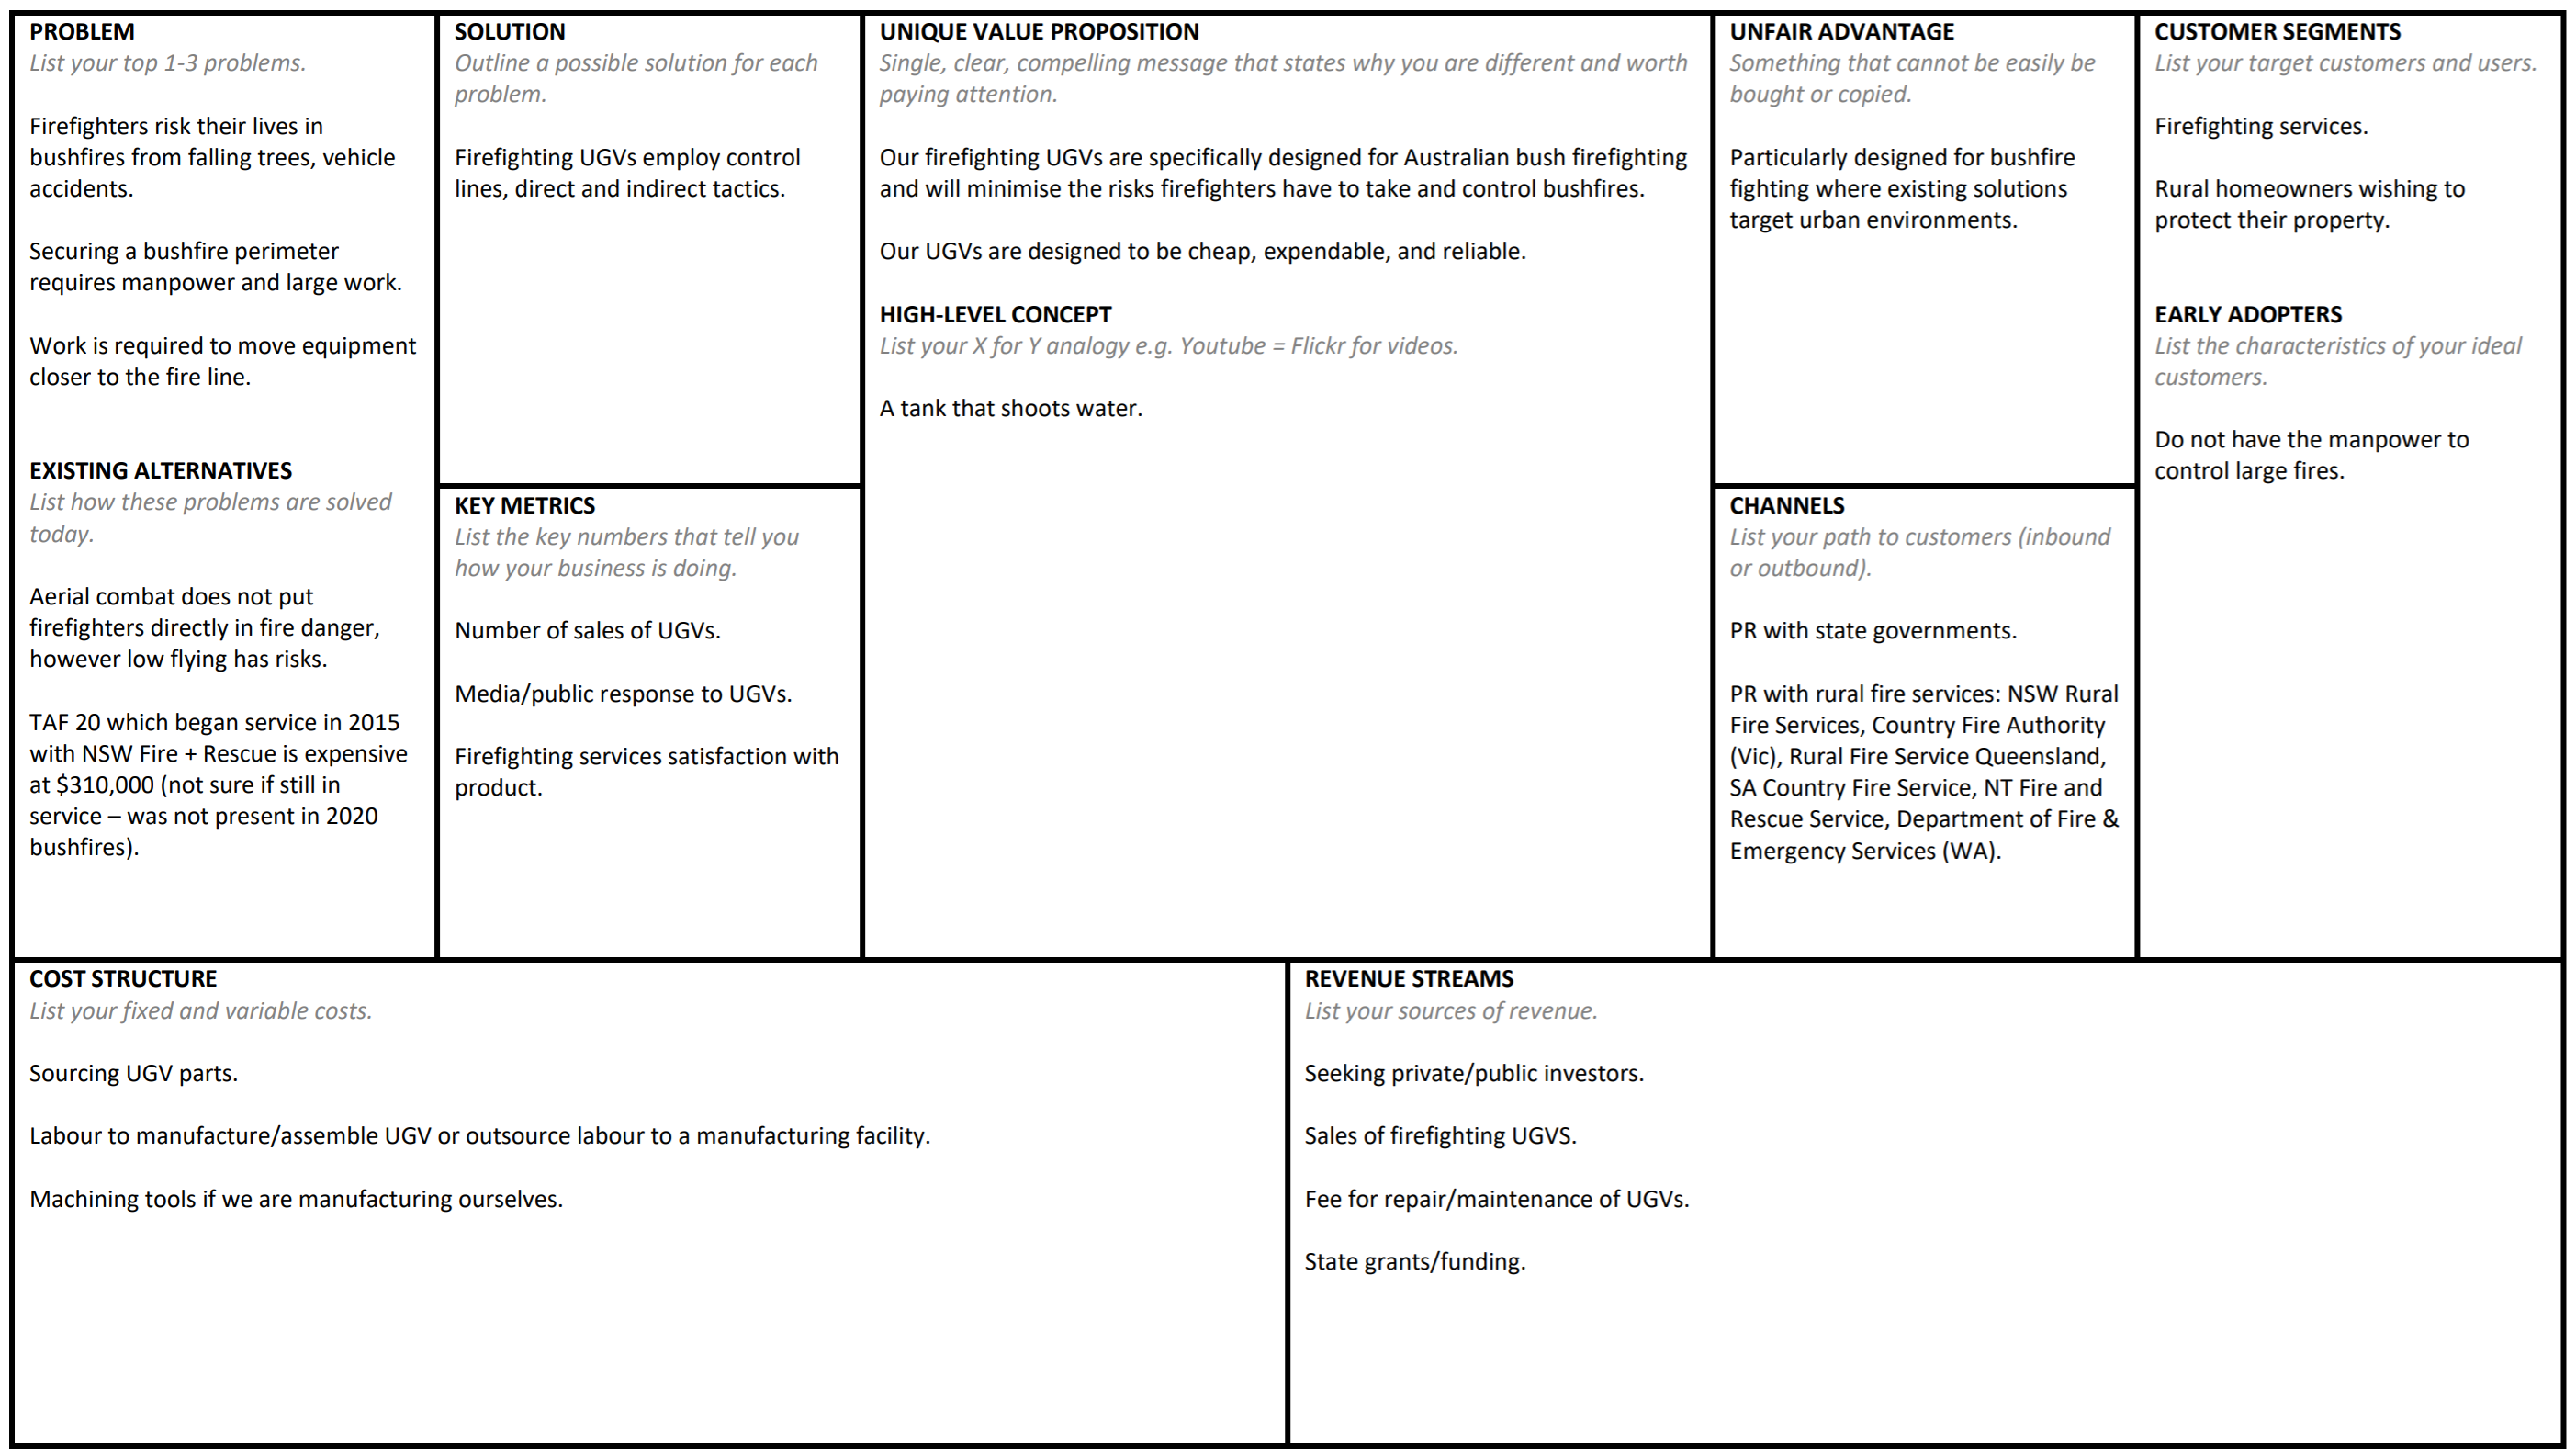
\includegraphics[width=\textwidth]{week2/lean_canvas_ugv.png}
		\caption{Firefighting UGV Lean Canvas}
		\label{fig:ugv_lean_canvas}
	\end{figure}

	\begin{figure}[h!]
		\centering
		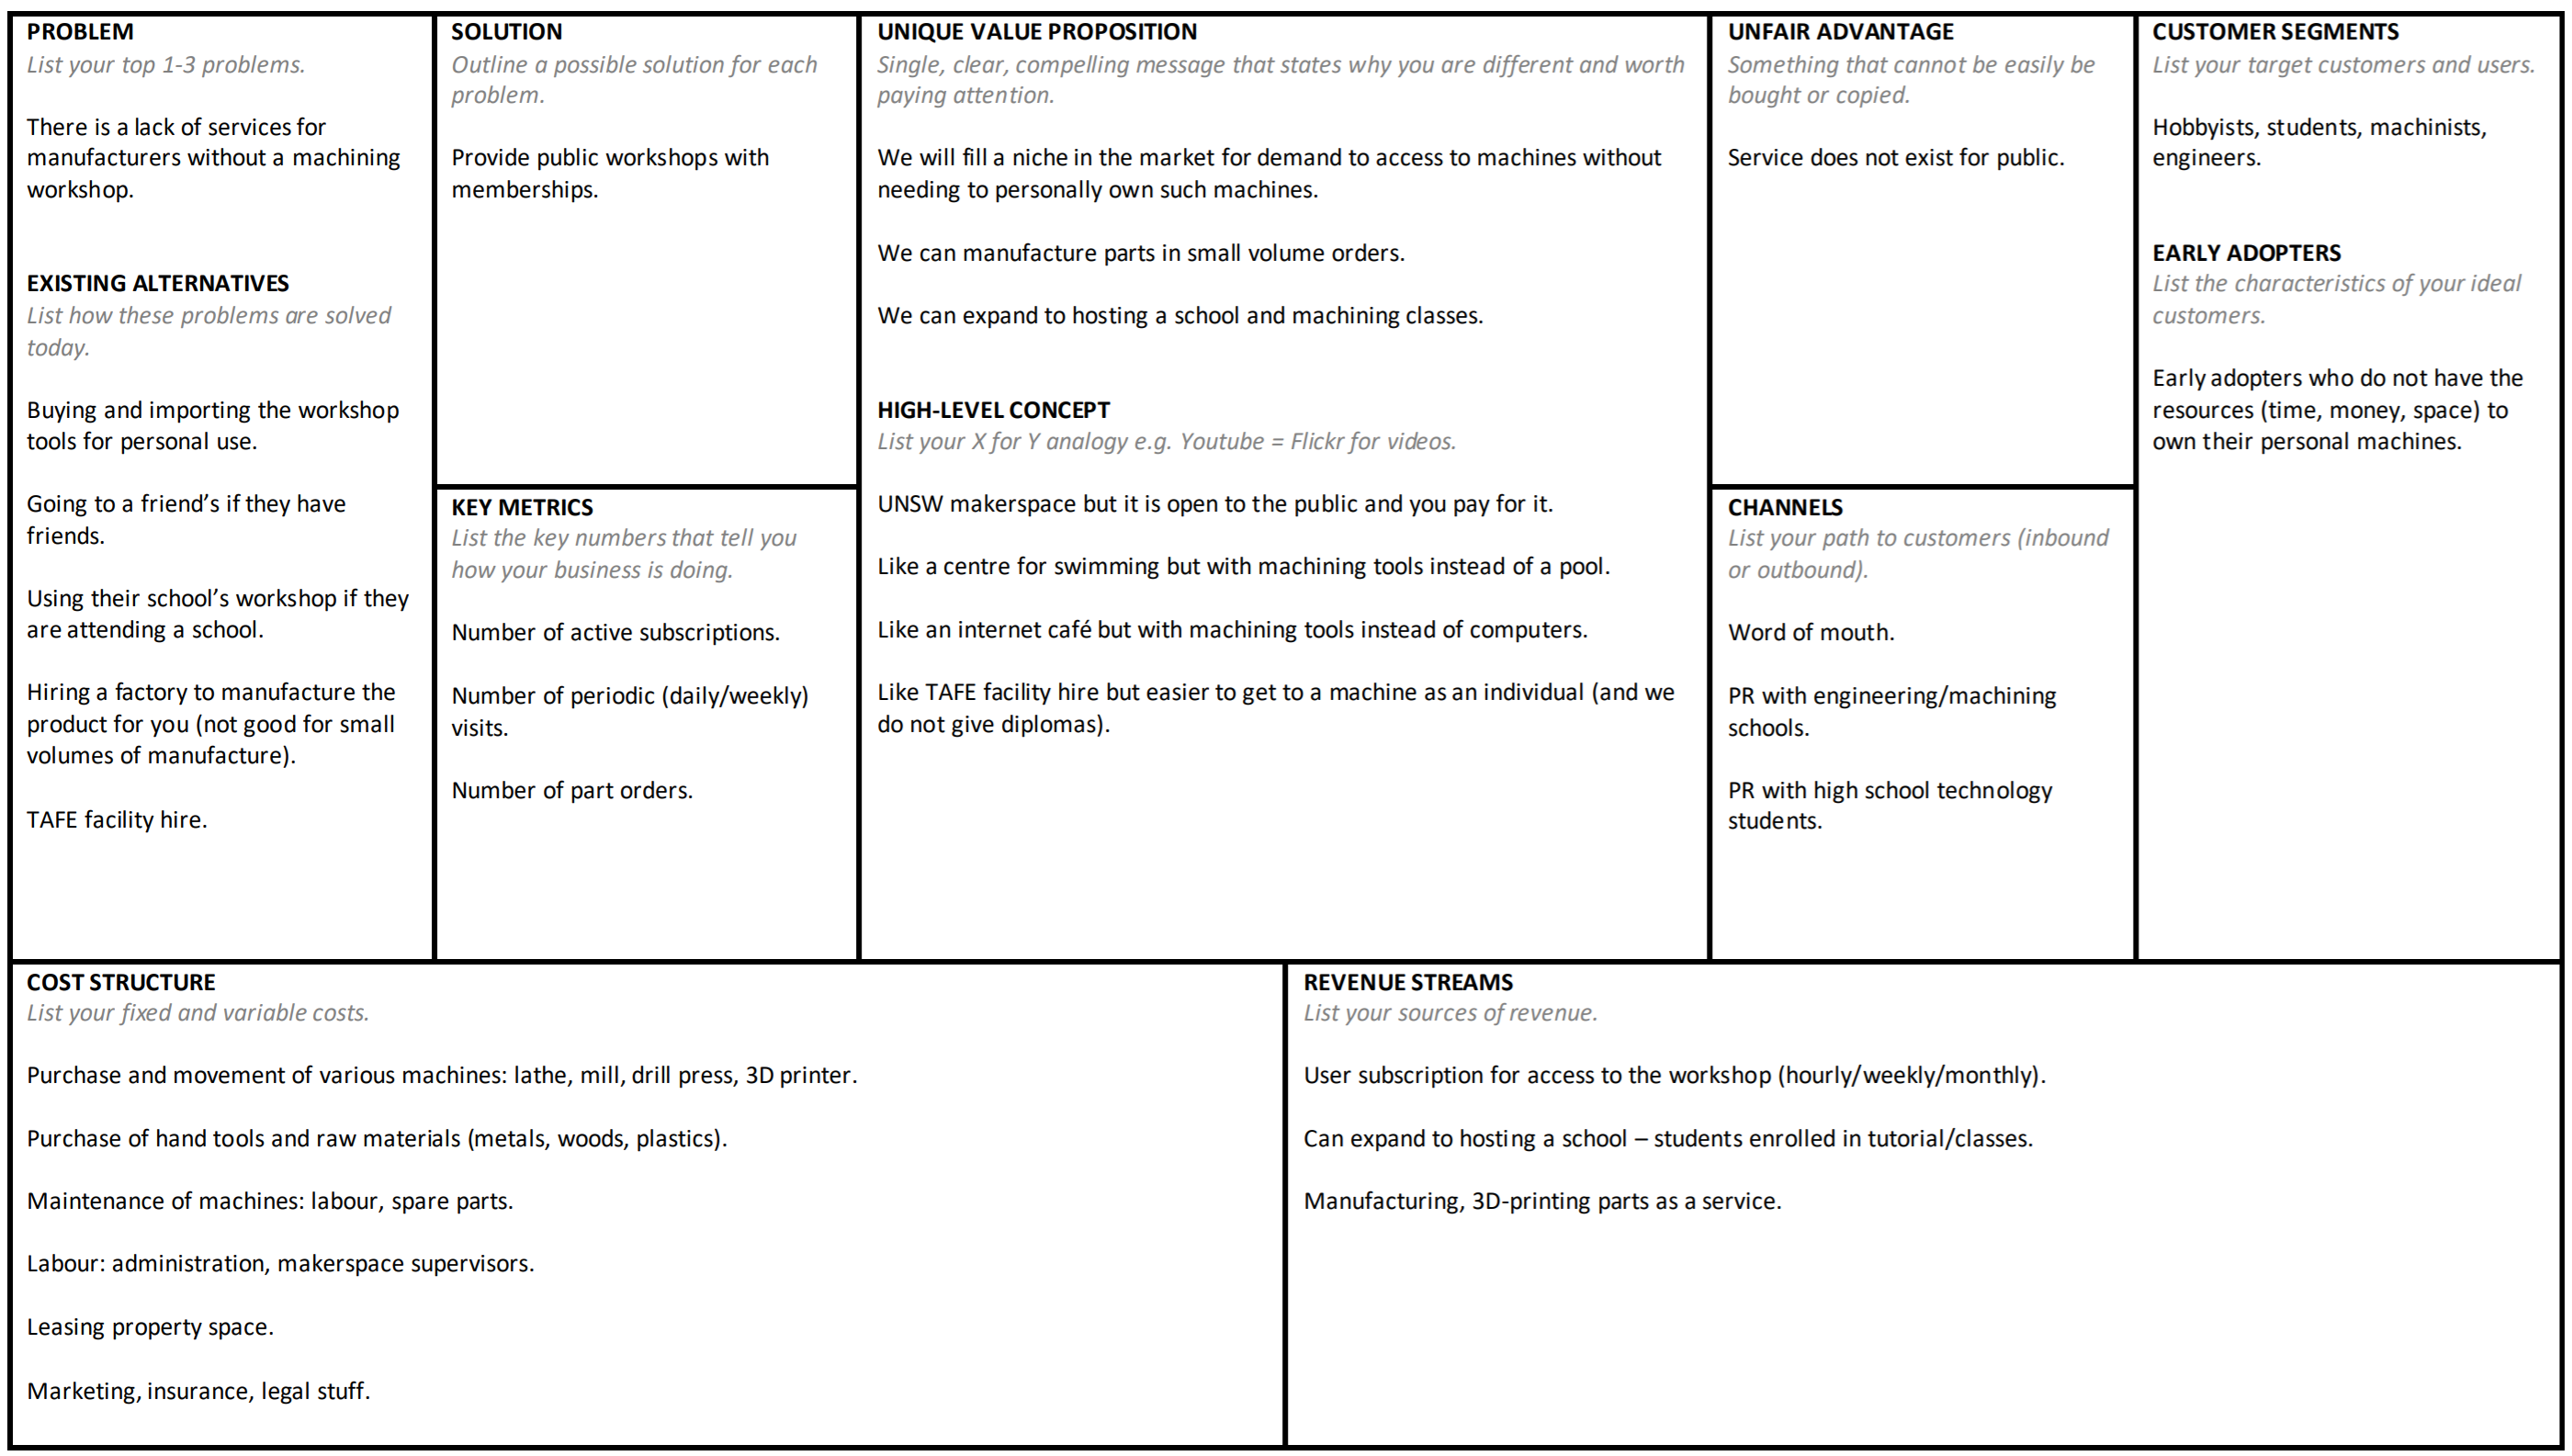
\includegraphics[width=\textwidth]{week2/lean_canvas_workshop.png}
		\caption{Machining Workshop Lean Canvas}
		\label{fig:workshop_lean_canvas}
	\end{figure}

\section{Week 3 Scribing}
\label{app:week3_scribe}
	
	Week 3 minutes (Figure \ref{fig:week3_scribe}).

	\begin{figure}[h!]
		\centering
		\fbox{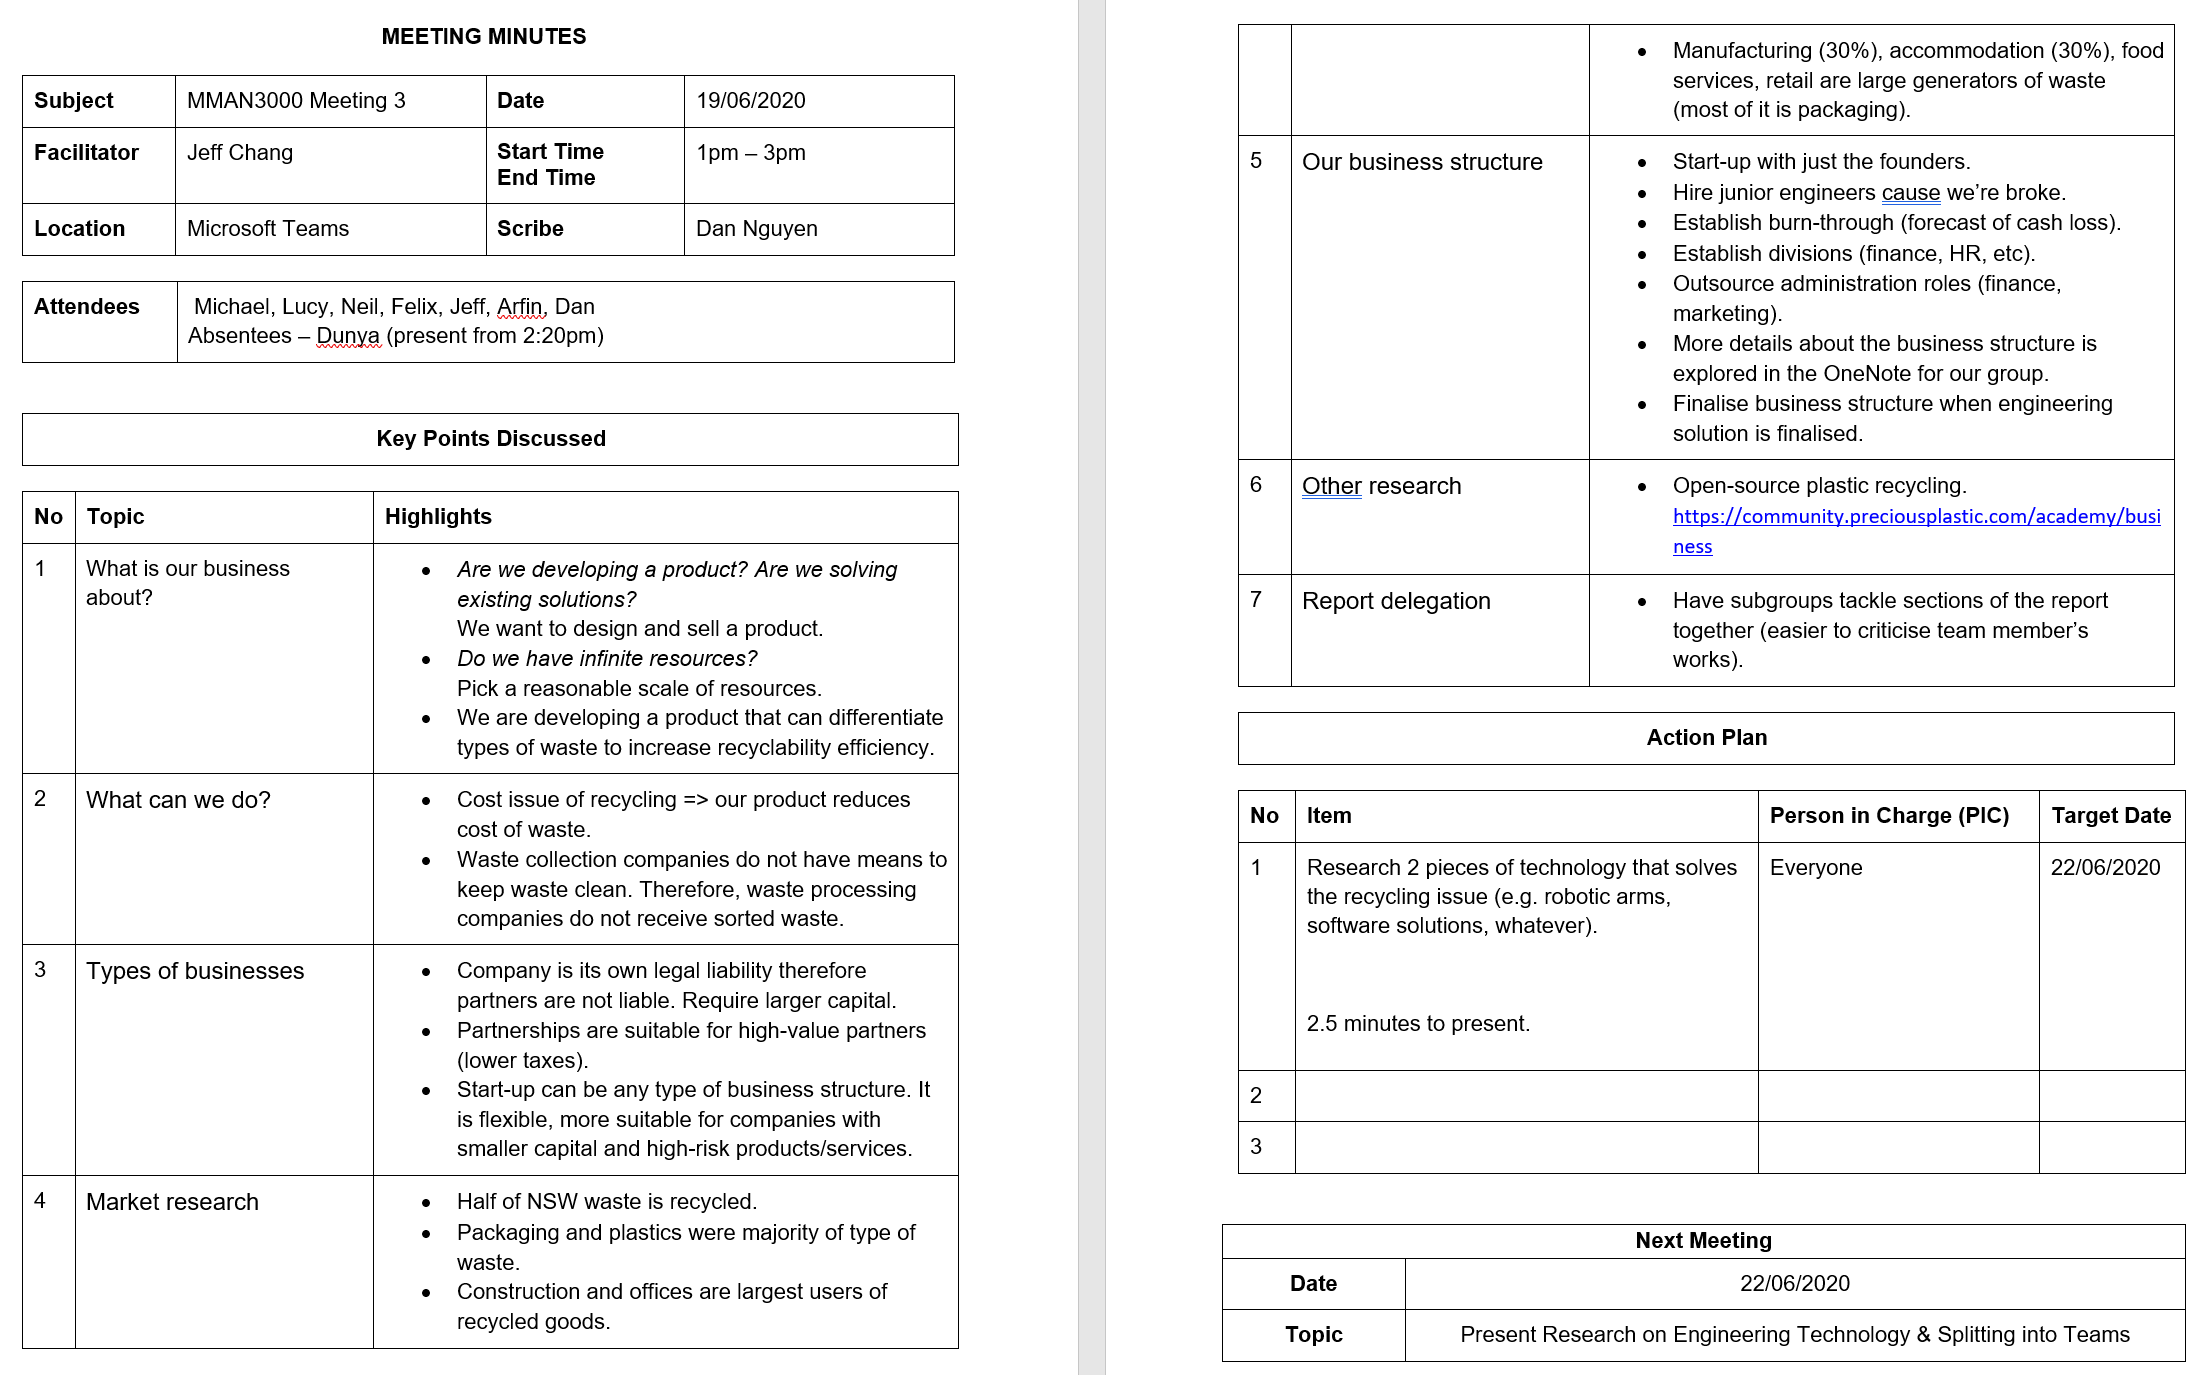
\includegraphics[width=0.98\textwidth]{week3/minutes.png}}
		\caption{Week 3 Minutes}
		\label{fig:week3_scribe}
	\end{figure}

\pagebreak

\section{Business Structures}
\label{app:business_structures}

	Business structure research from week 3 in Figure \ref{fig:business_structure}.

	\begin{figure}[h!]
		\centering
		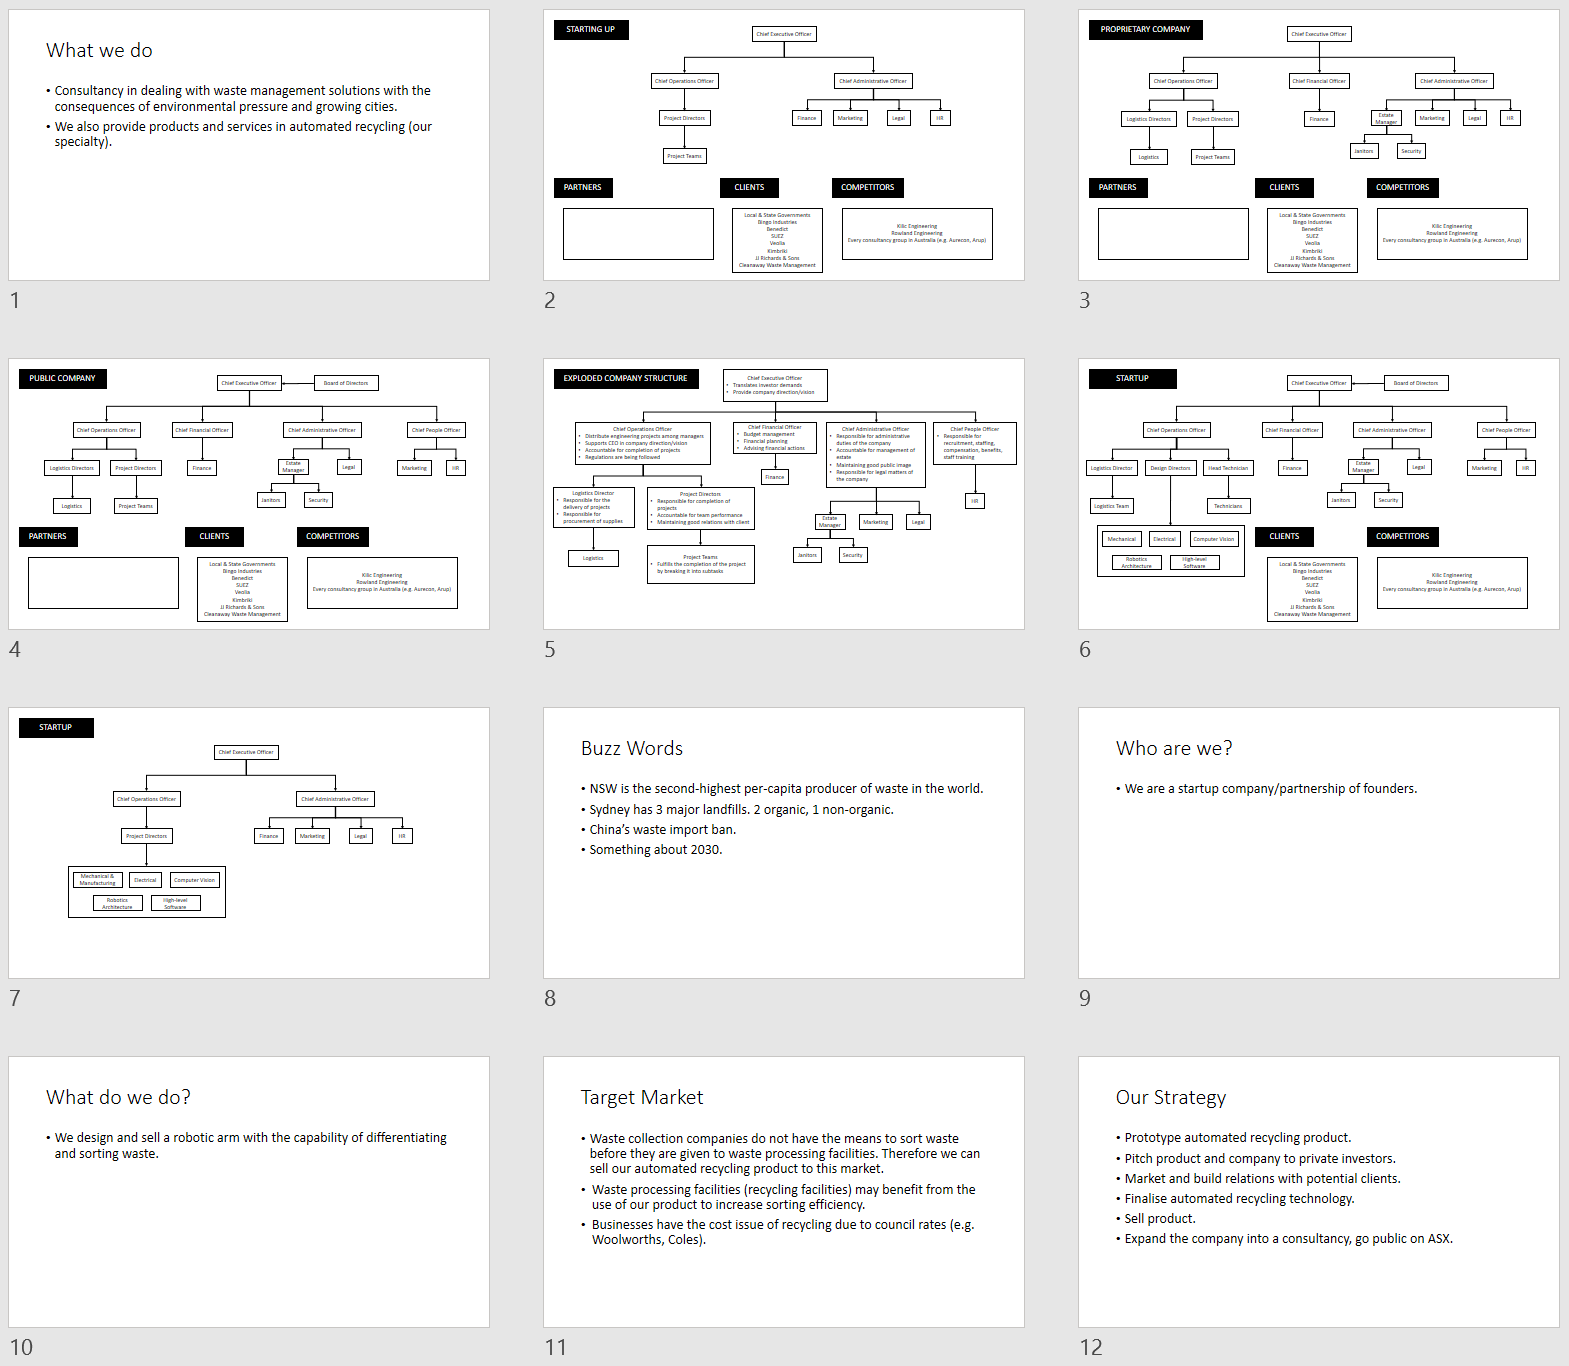
\includegraphics[width=\textwidth]{week3/business_structure.png}
		\caption{Business Structure Work}
		\label{fig:business_structure}
	\end{figure}

\pagebreak

\section{Week 4 Chairing}
\label{app:week4_chair}

	Week 4 chairing Monday agenda (Figure \ref{fig:week4_agenda1}) and Friday agenda (Figure \ref{fig:week4_agenda2}).

	\begin{figure}[h!]
		\centering
		\fbox{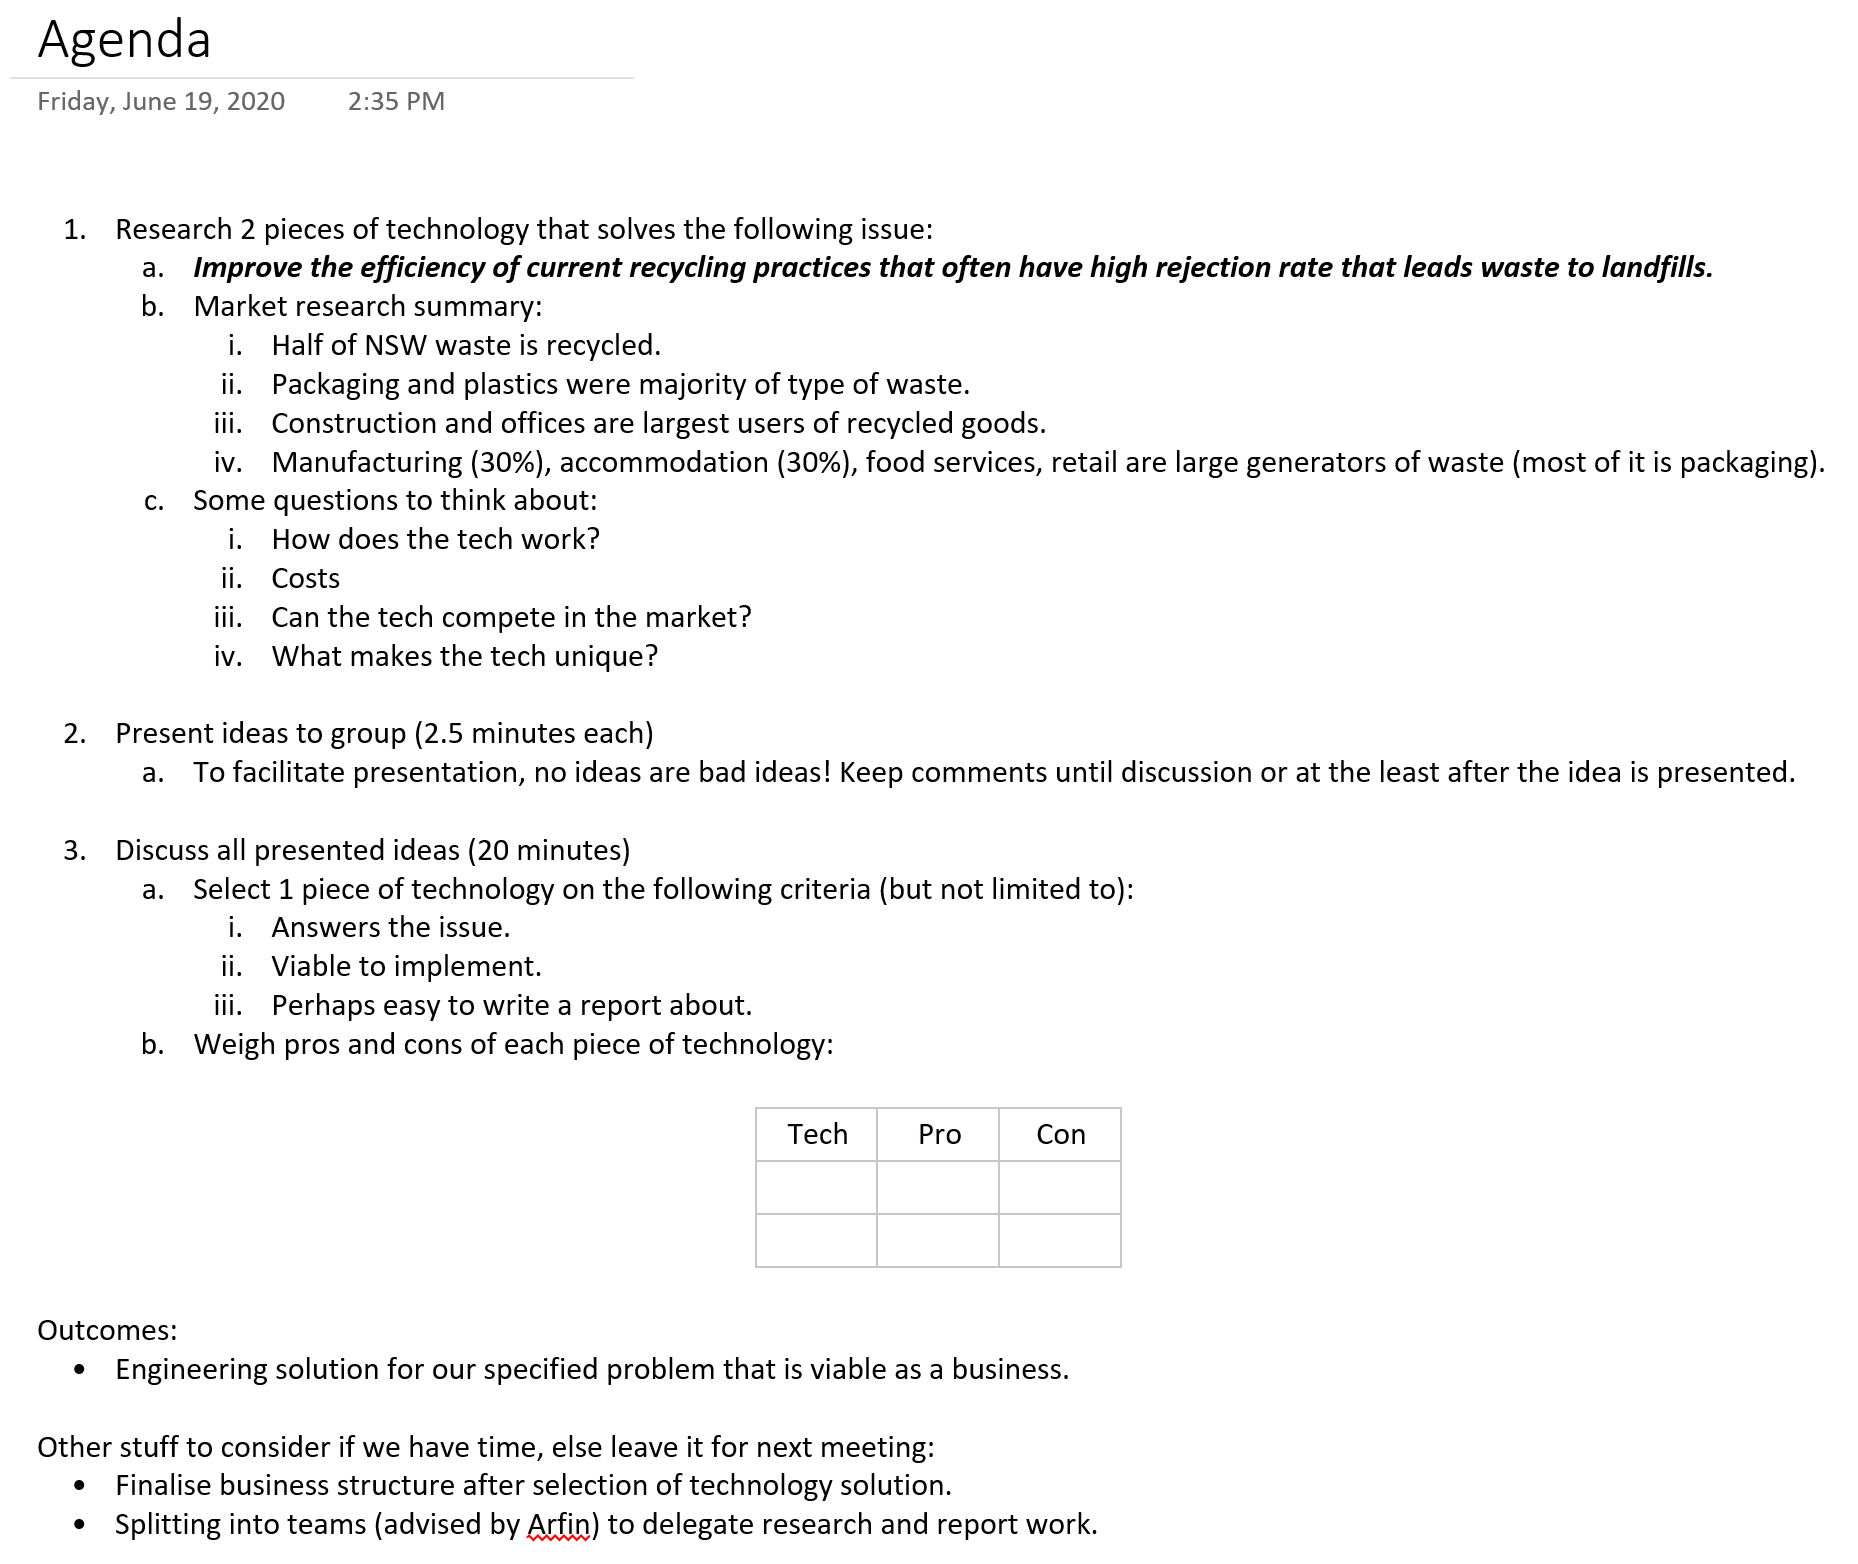
\includegraphics[width=0.8\textwidth]{week4/agenda1.png}}
		\caption{Week 4 Monday Agenda}
		\label{fig:week4_agenda1}
	\end{figure}

	\begin{figure}[h!]
		\centering
		\fbox{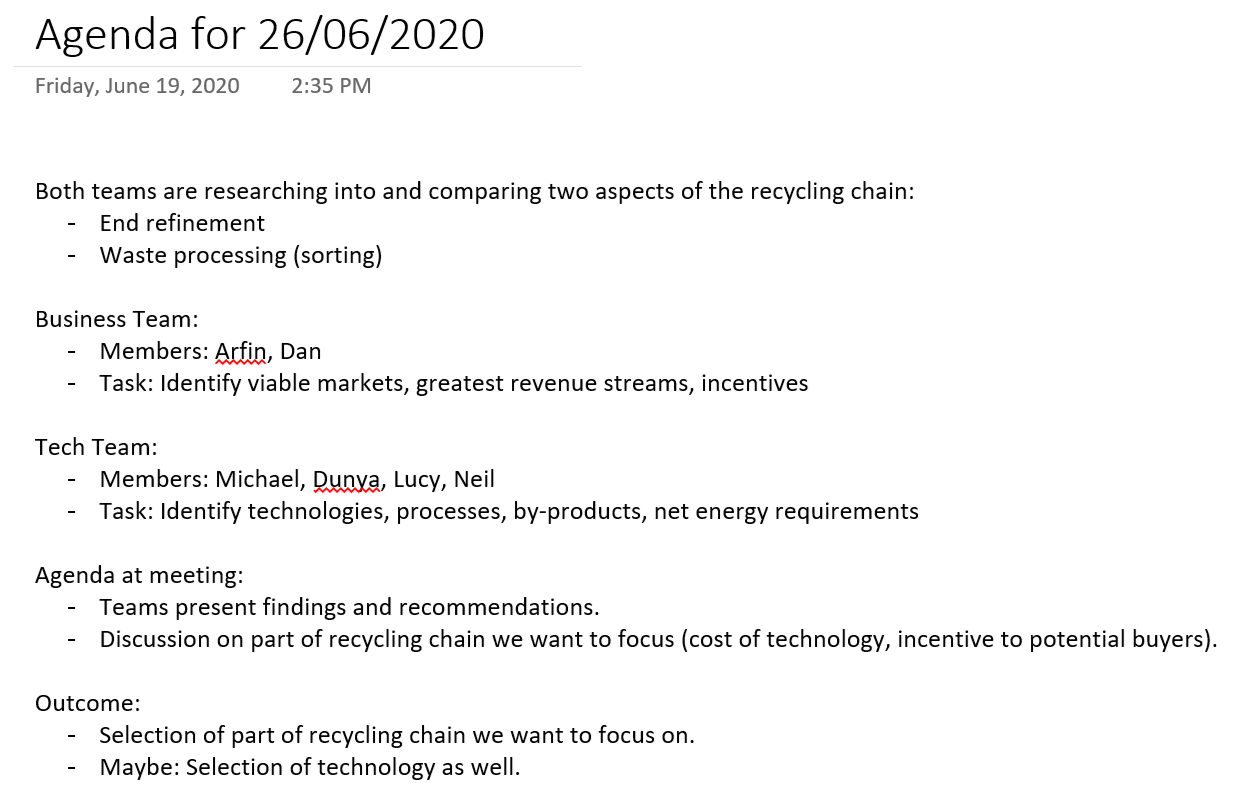
\includegraphics[width=0.8\textwidth]{week4/agenda2.png}}
		\caption{Week 4 Friday Agenda}
		\label{fig:week4_agenda2}
	\end{figure}

\pagebreak

\section{Technology Research}
\label{app:technology_research}

	Technology research conducted in week 4 in Figure \ref{fig:technology_research}.

	\begin{figure}[h!]
		\centering
		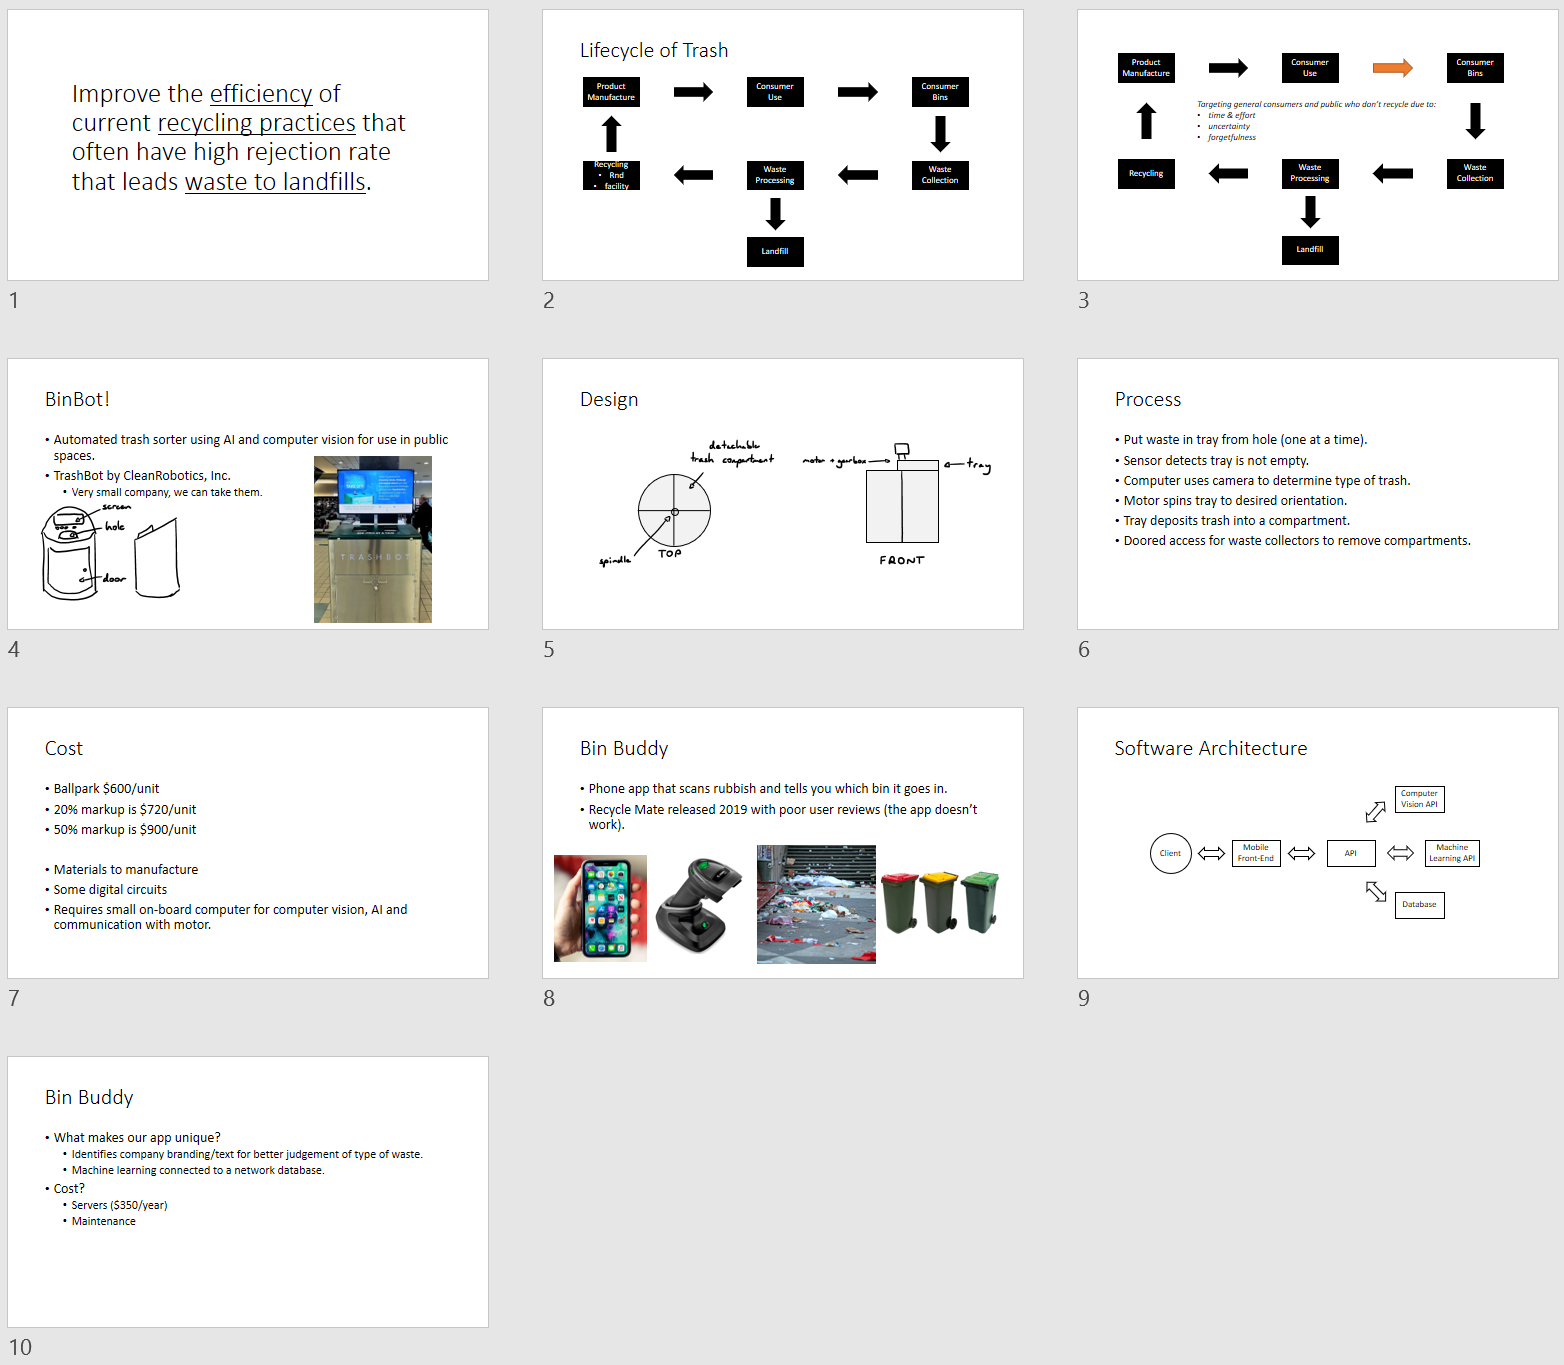
\includegraphics[width=\textwidth]{week4/technology_research.png}
		\caption{Technology Research}
		\label{fig:technology_research}
	\end{figure}

\pagebreak

\section{Market Research}
\label{app:market_research}

	Market research conducted in week 4 in Figures \ref{fig:business_research}, \ref{fig:waste_management}, \ref{fig:resource_recovery}, \ref{fig:paper}, \ref{fig:glass}, \ref{fig:plastic}, \ref{fig:rubber}.

	\begin{figure}[h!]
		\centering
		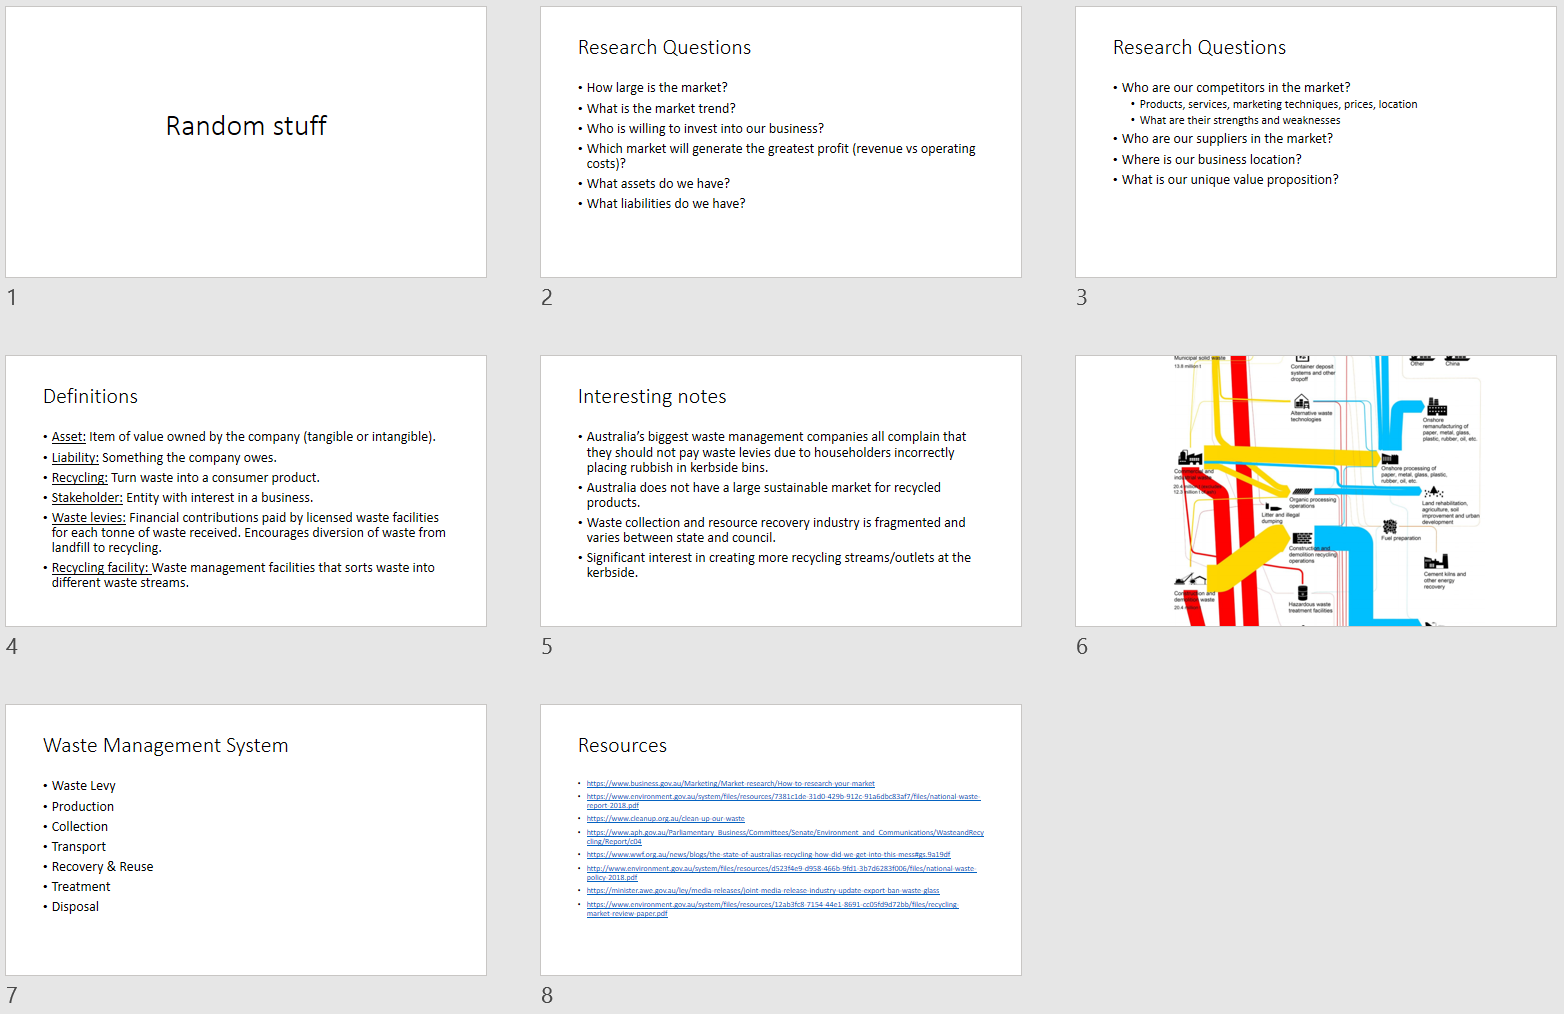
\includegraphics[width=\textwidth]{week4/business_team_research.png}
		\caption{Market Research Questions}
		\label{fig:business_research}
	\end{figure}

	\begin{figure}[h!]
		\centering
		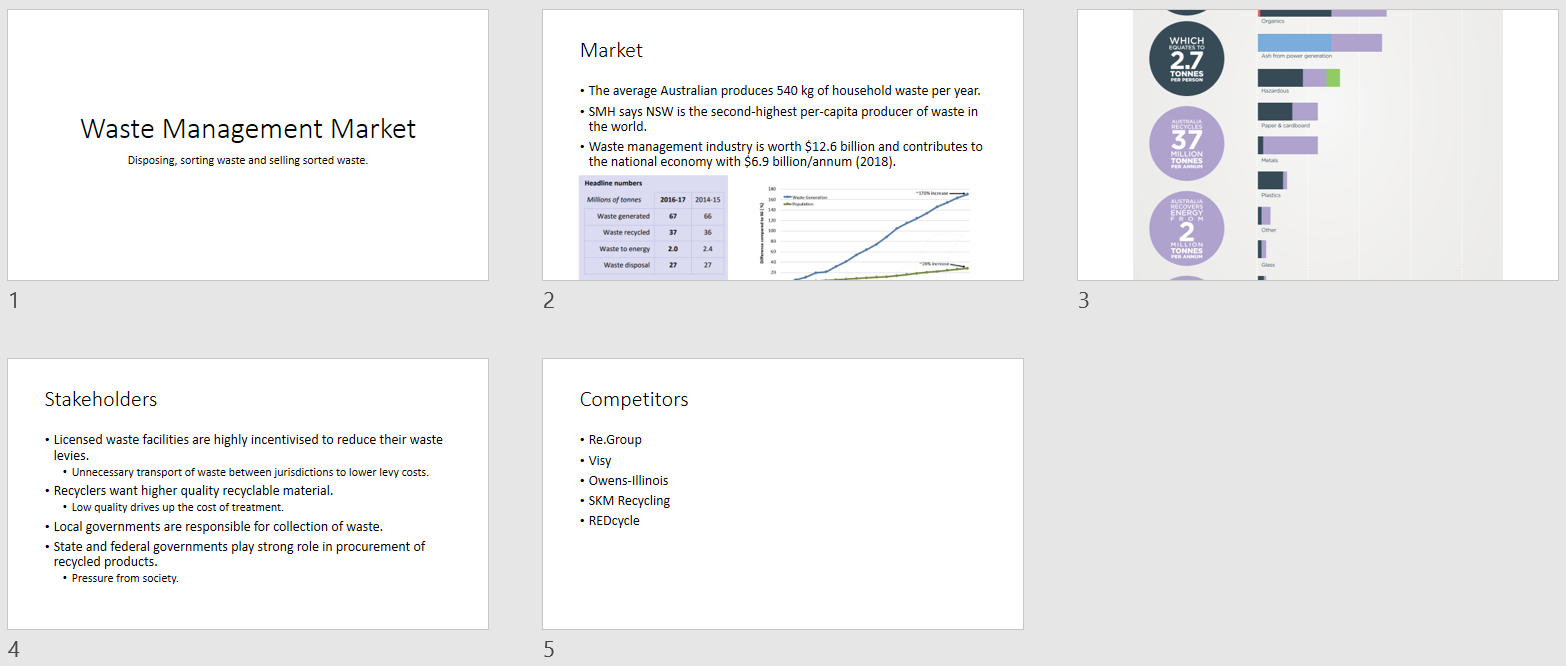
\includegraphics[width=\textwidth]{week4/business_research_waste_management.png}
		\caption{Waste Management Market Research}
		\label{fig:waste_management}
	\end{figure}

	\begin{figure}[h!]
		\centering
		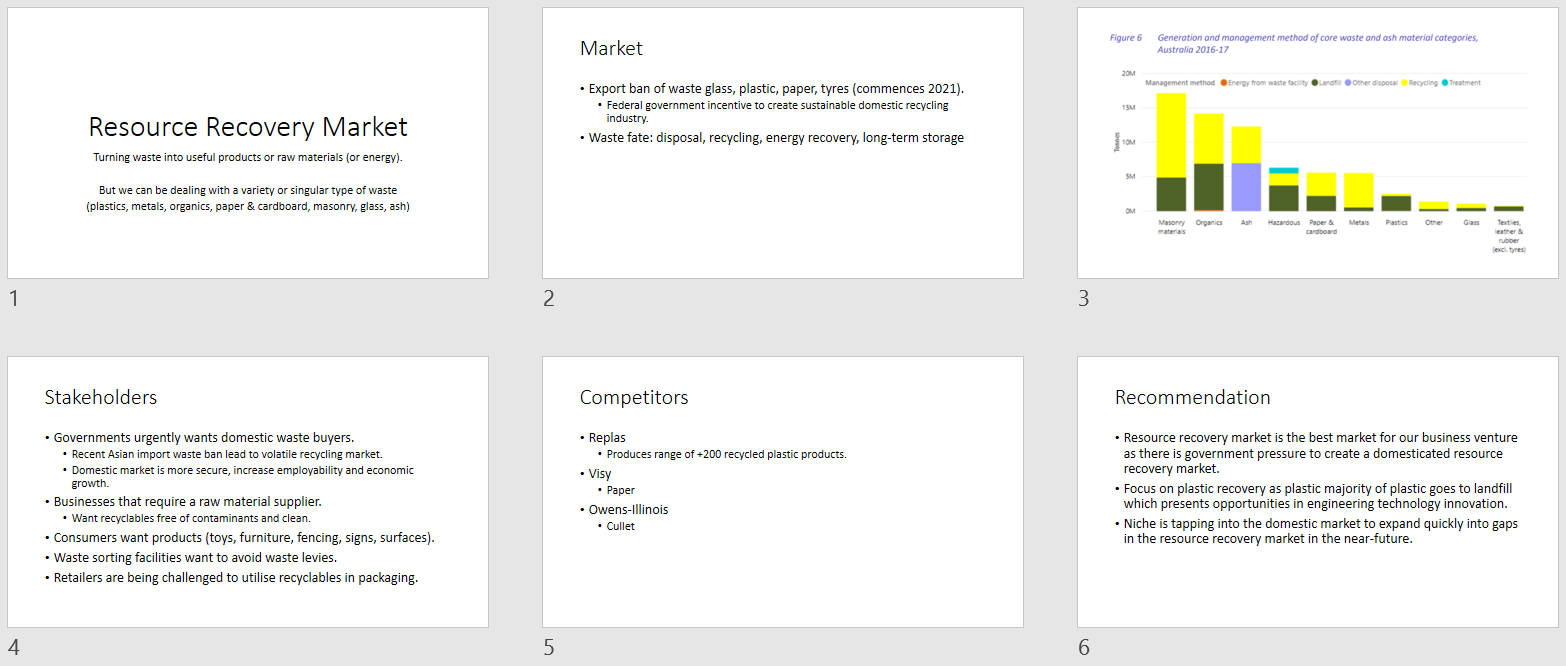
\includegraphics[width=\textwidth]{week4/business_research_resource_recovery.png}
		\caption{Resource Recovery Market Research}
		\label{fig:resource_recovery}
	\end{figure}

	\begin{figure}[h!]
		\centering
		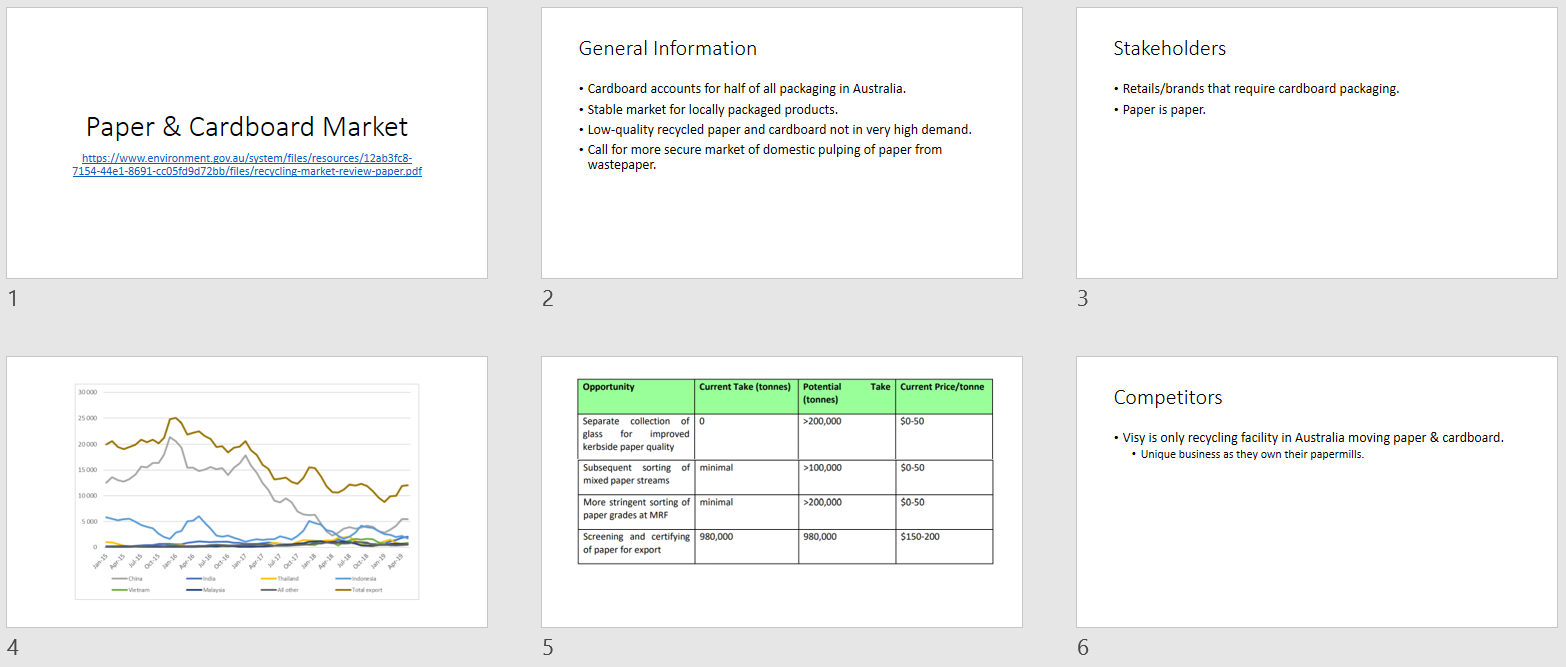
\includegraphics[width=\textwidth]{week4/business_research_paper.png}
		\caption{Paper Market Research}
		\label{fig:paper}
	\end{figure}

	\begin{figure}[h!]
		\centering
		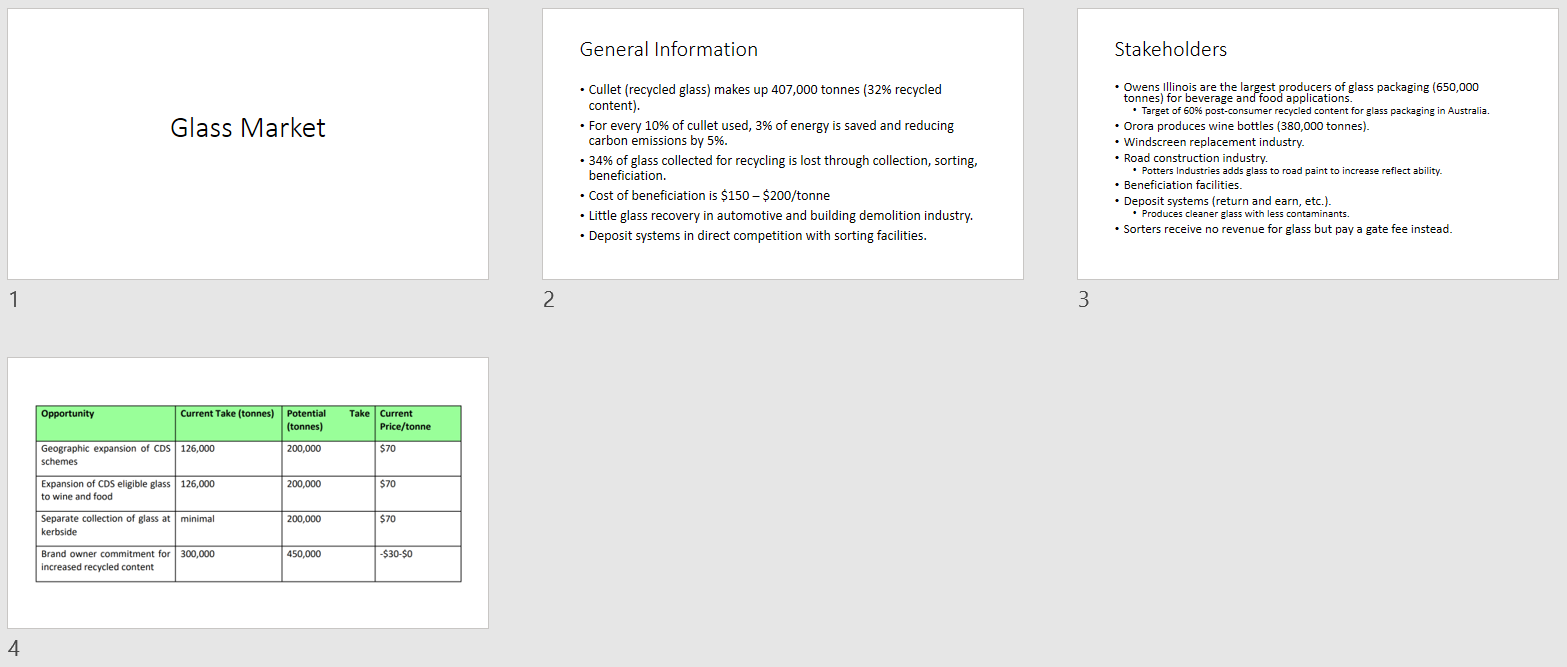
\includegraphics[width=\textwidth]{week4/business_research_glass.png}
		\caption{Glass Market Research}
		\label{fig:glass}
	\end{figure}

	\begin{figure}[h!]
		\centering
		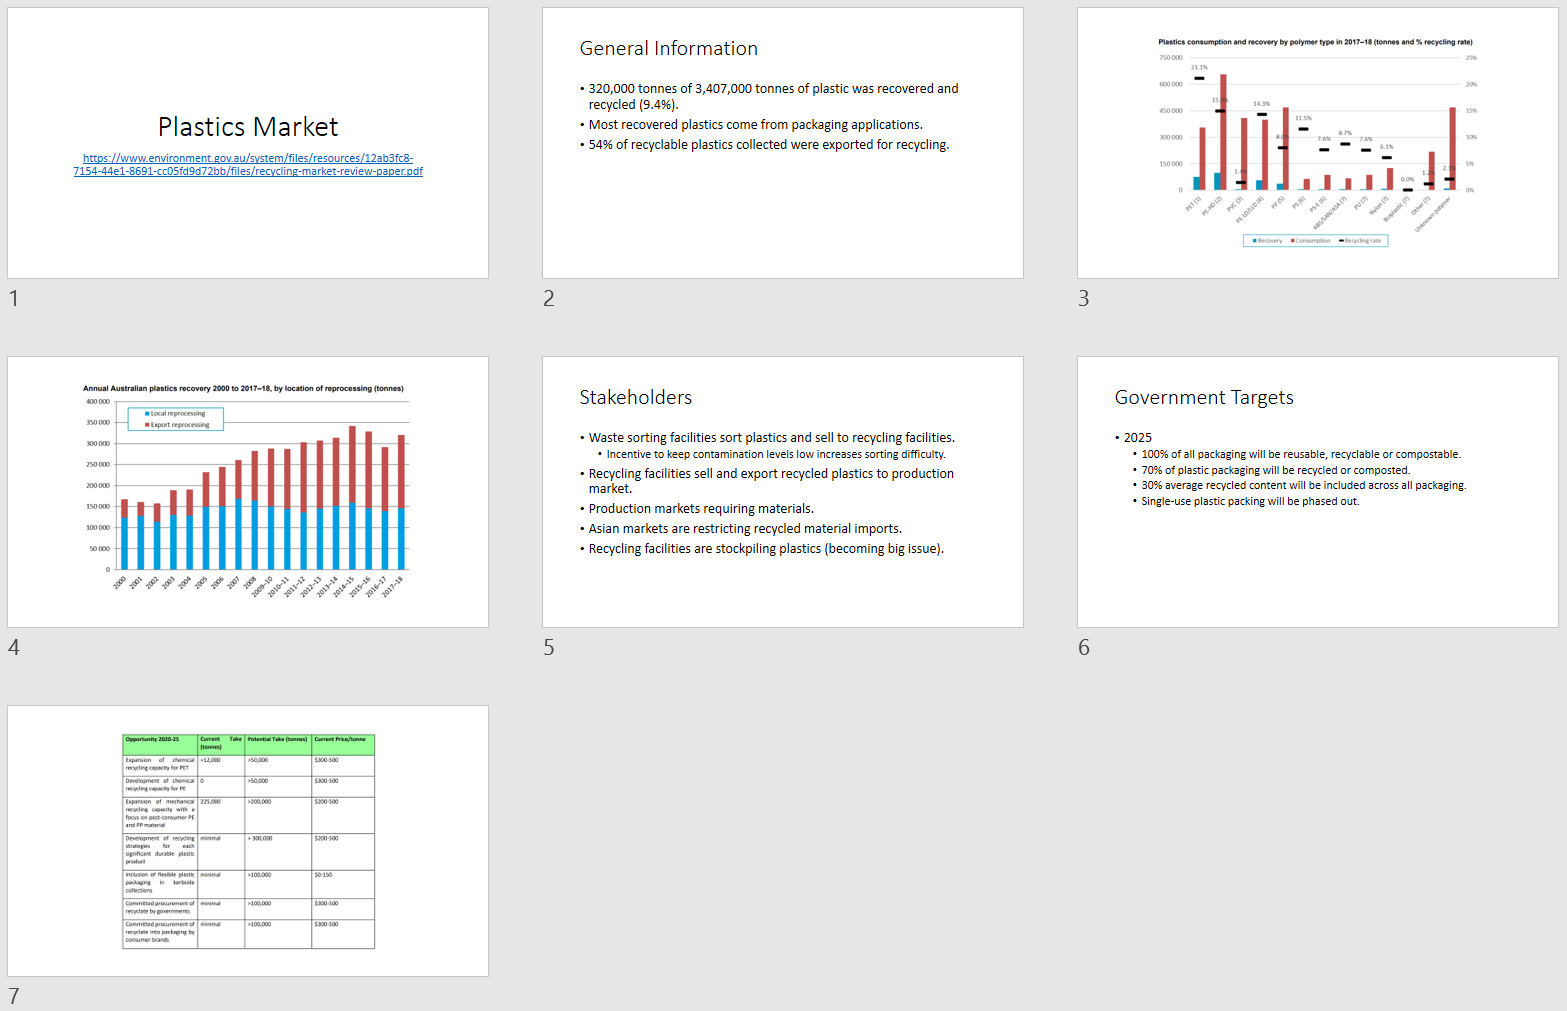
\includegraphics[width=\textwidth]{week4/business_research_plastic.png}
		\caption{Plastic Market Research}
		\label{fig:plastic}
	\end{figure}

	\begin{figure}[h!]
		\centering
		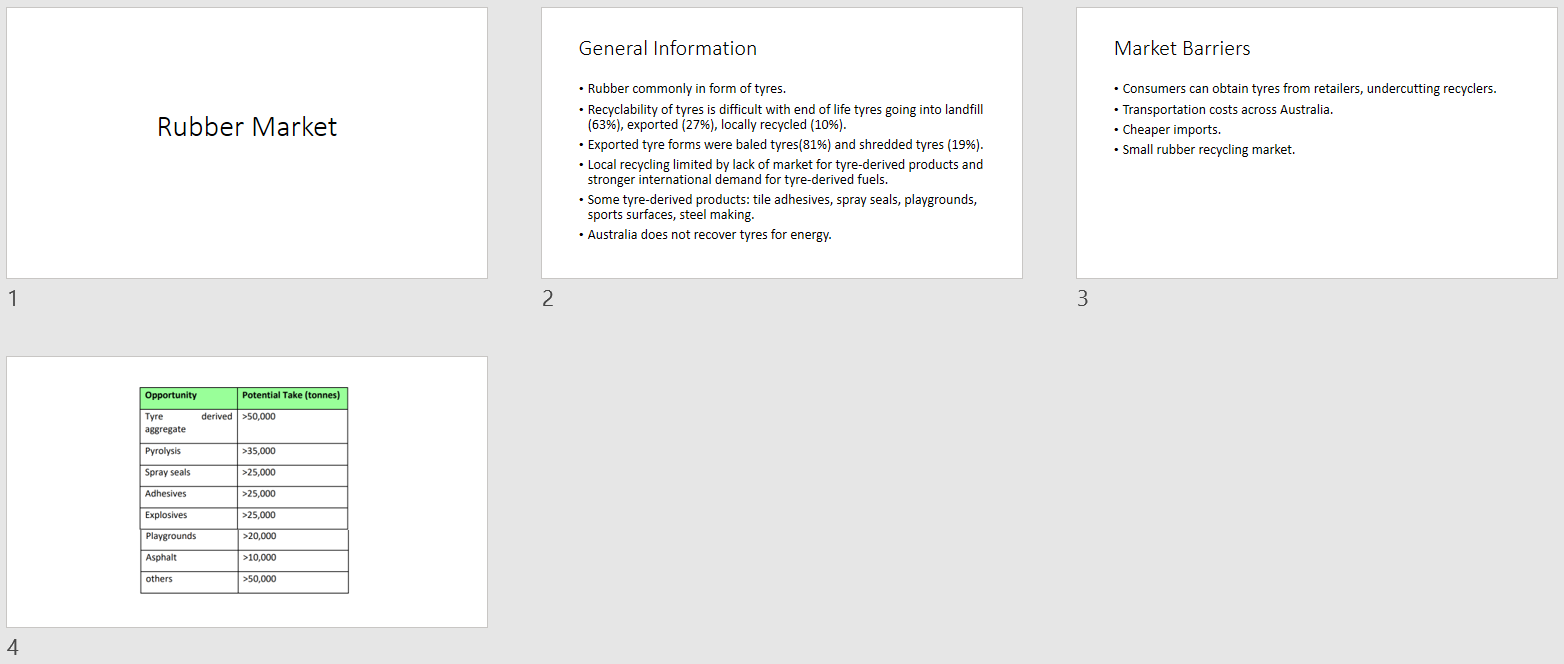
\includegraphics[width=\textwidth]{week4/business_research_rubber.png}
		\caption{Rubber Market Research}
		\label{fig:rubber}
	\end{figure}

\pagebreak

\section{Week 7 Scribing}
\label{app:week7_scribe}

	Week 7 minutes (Figure \ref{fig:week7_scribe}).

	\begin{figure}[h!]
		\centering
		\fbox{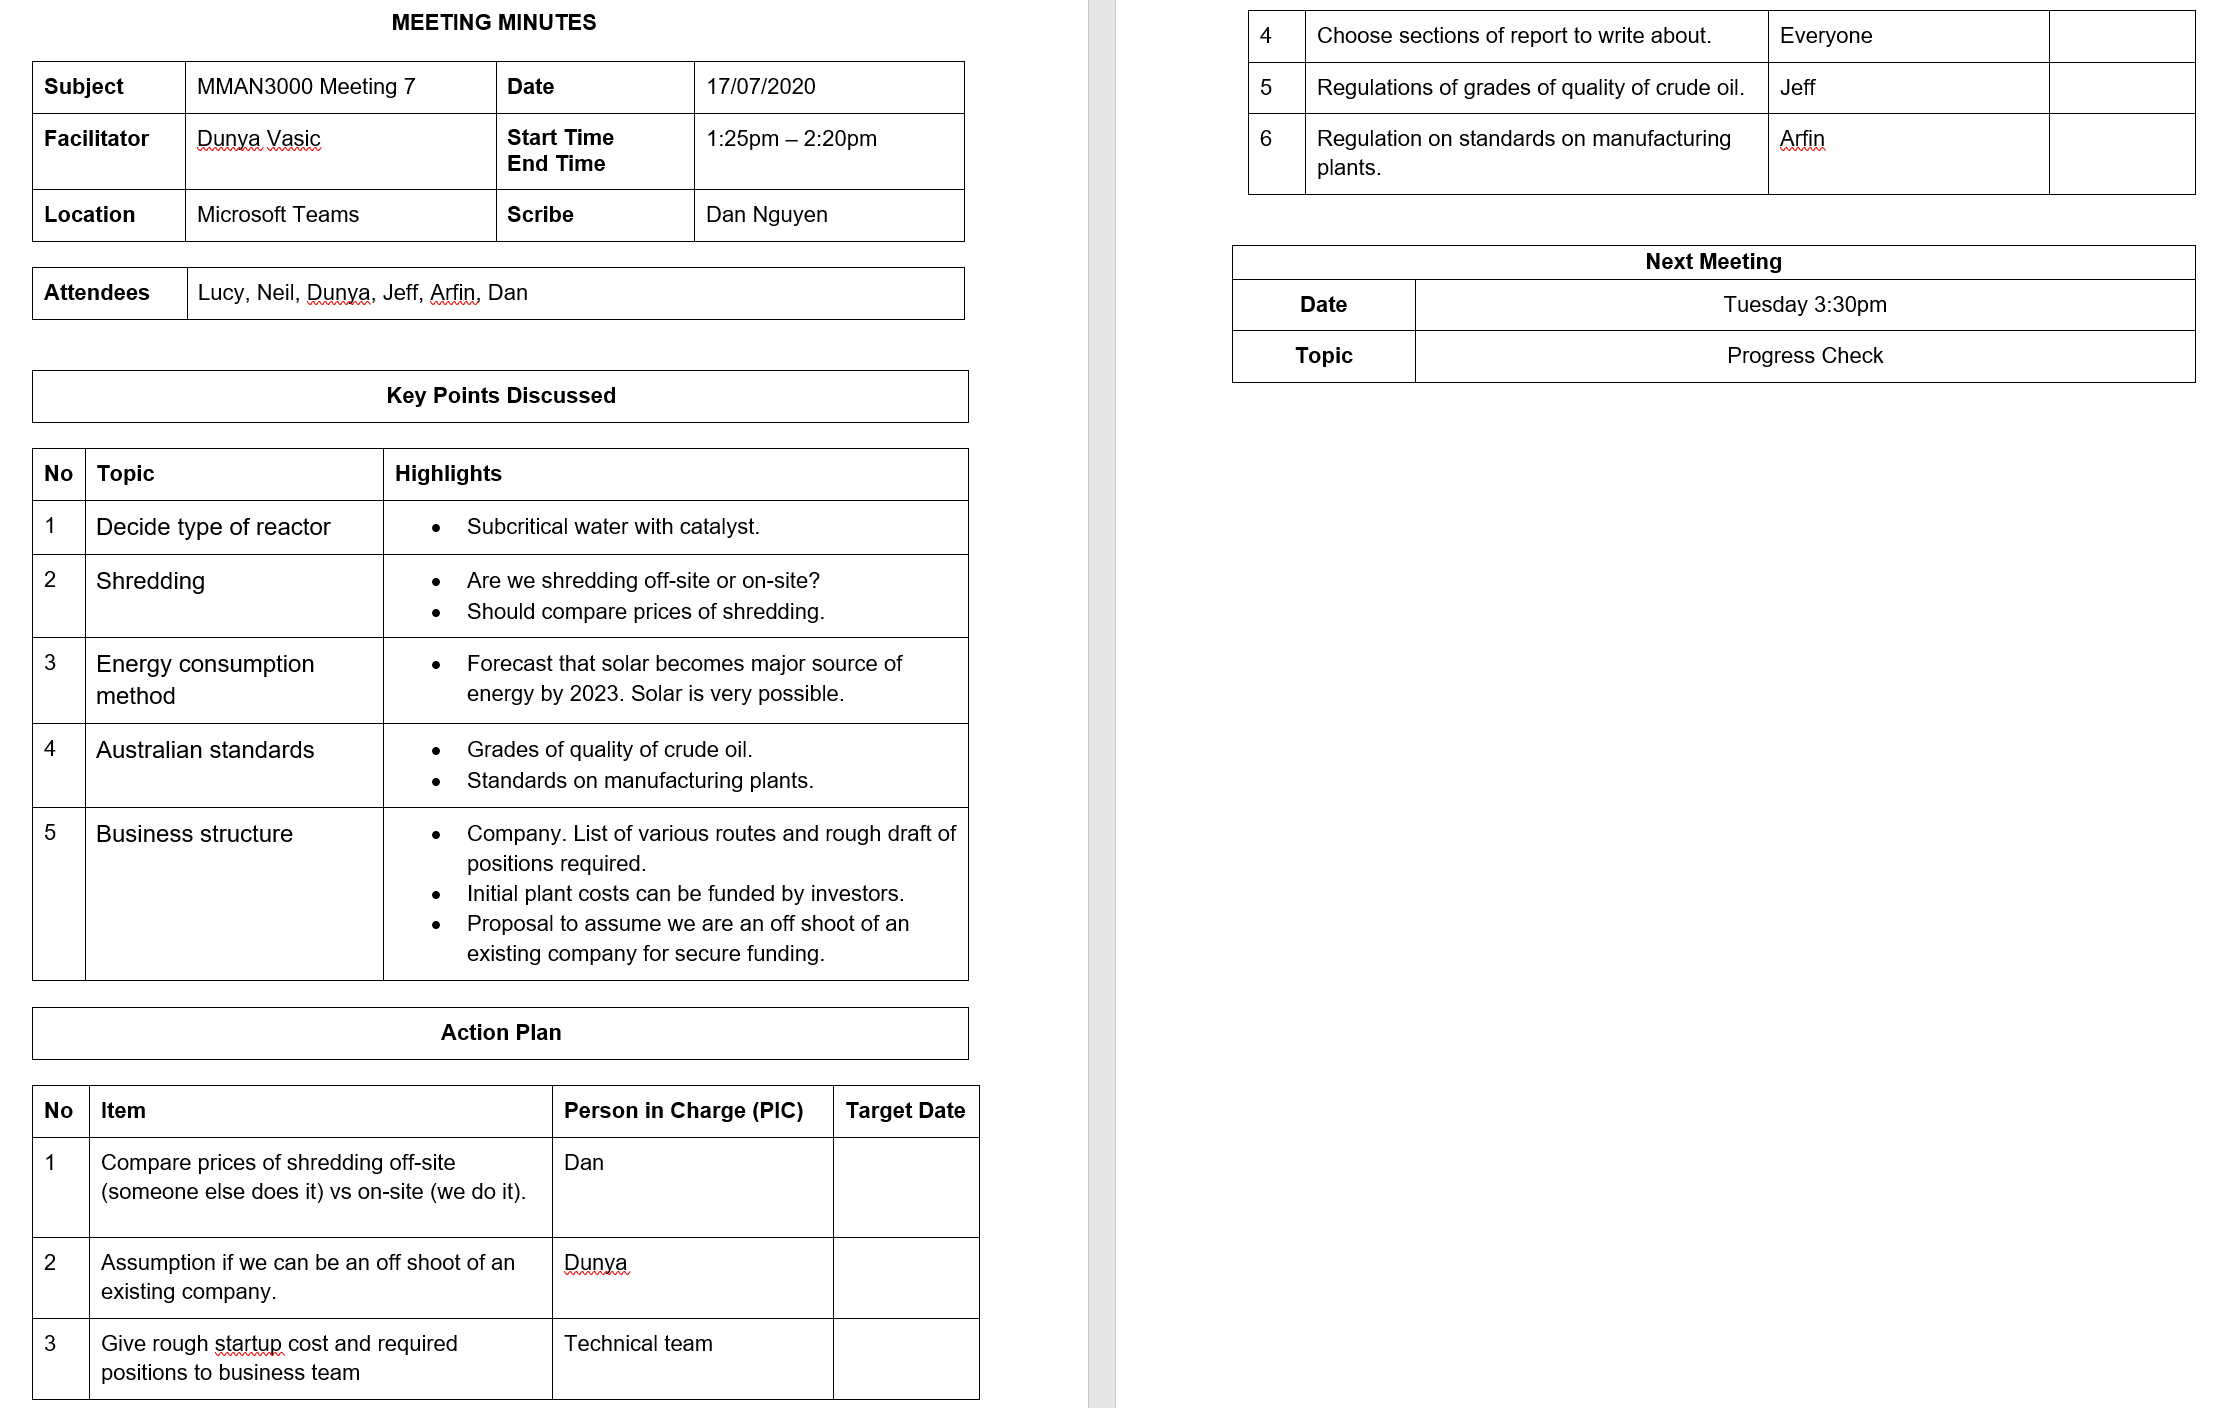
\includegraphics[width=0.98\textwidth]{week7/week7_scribe.png}}
		\caption{Week 7 Minutes}
		\label{fig:week7_scribe}
	\end{figure}

\pagebreak

\section{Shredding Prices}
\label{app:shred}

	On-site shredding cost from week 7 in Figure \ref{fig:shredder_cost}.

	\begin{figure}[h!]
		\centering
		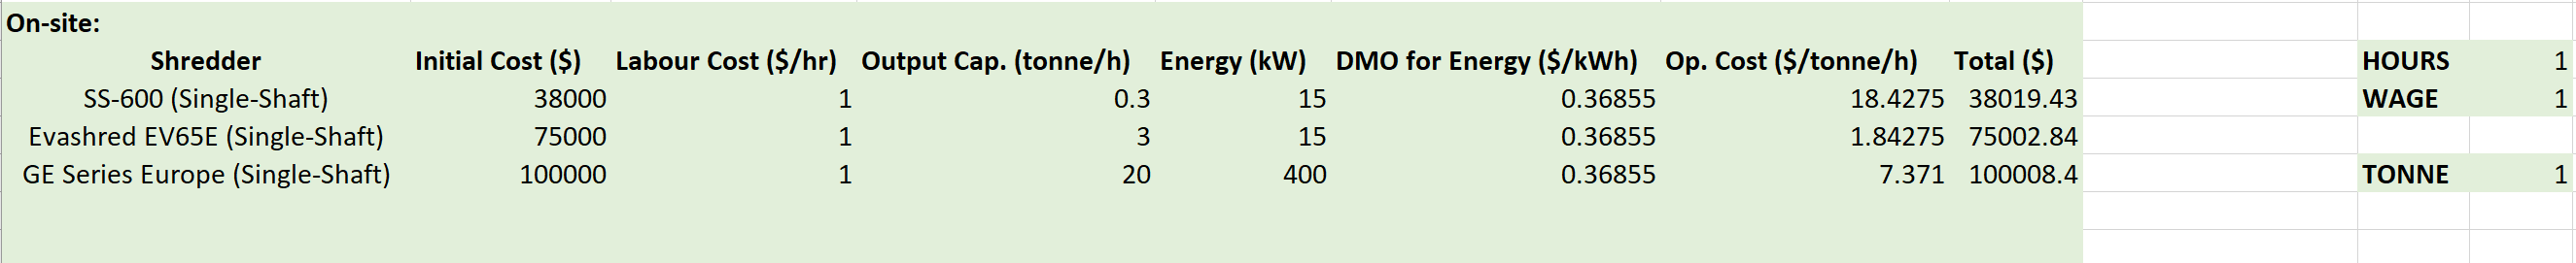
\includegraphics[width=\textwidth]{week7/shredder_cost.png}
		\caption{On-site Shredding Cost}
		\label{fig:shredder_cost}
	\end{figure}

	Comparison between granulator and shredder in Figure \ref{fig:gran_vs_shred}.

	\begin{figure}[h!]
		\centering
		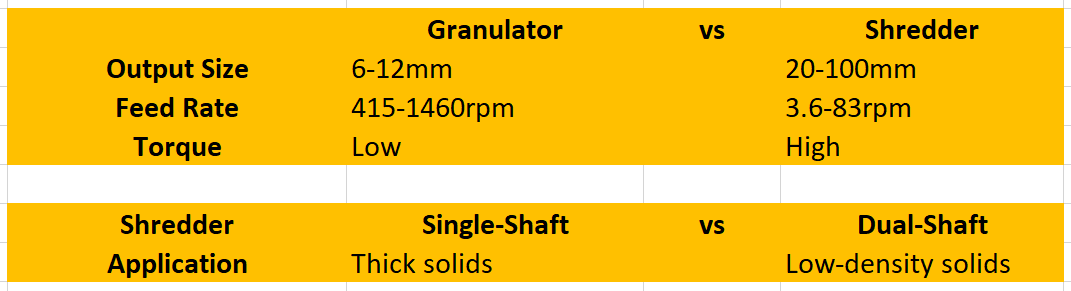
\includegraphics[width=10cm]{week7/granulator_vs_shredder.png}
		\caption{Granulator vs Shredder}
		\label{fig:gran_vs_shred}
	\end{figure}

\pagebreak

\section{Market Share Analysis}
\label{app:market_share}

	Market share analysis into major domestic plastic resource recovery companies (Figures \ref{fig:market_share} and \ref{fig:accepted_products}).

	\begin{figure}[h!]
		\centering
		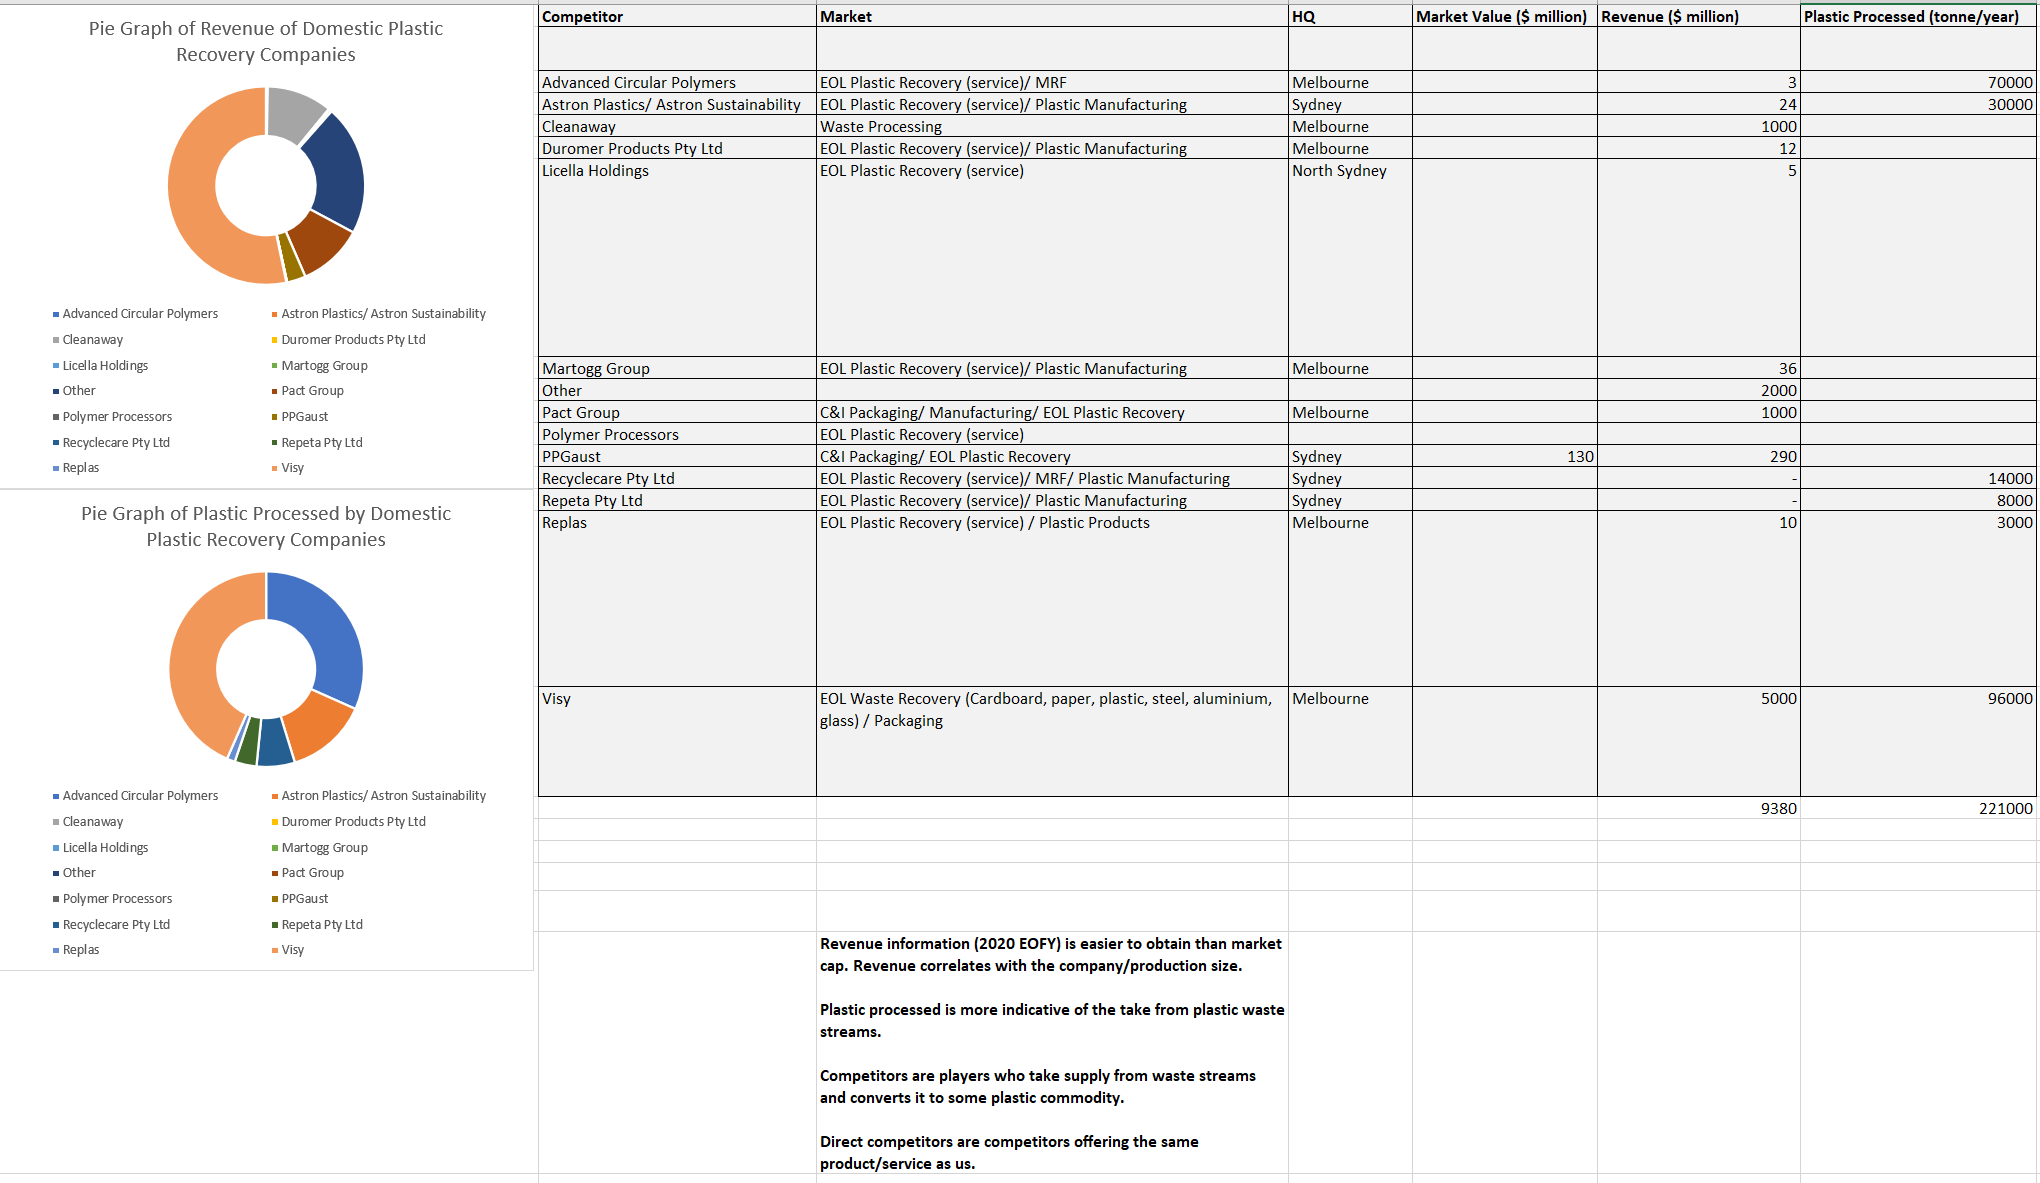
\includegraphics[width=\textwidth]{week7/domestic_plastic_resource_recovery_market_share.png}
		\caption{Market Share Analysis}
		\label{fig:market_share}
	\end{figure}

	\begin{figure}[h!]
		\centering
		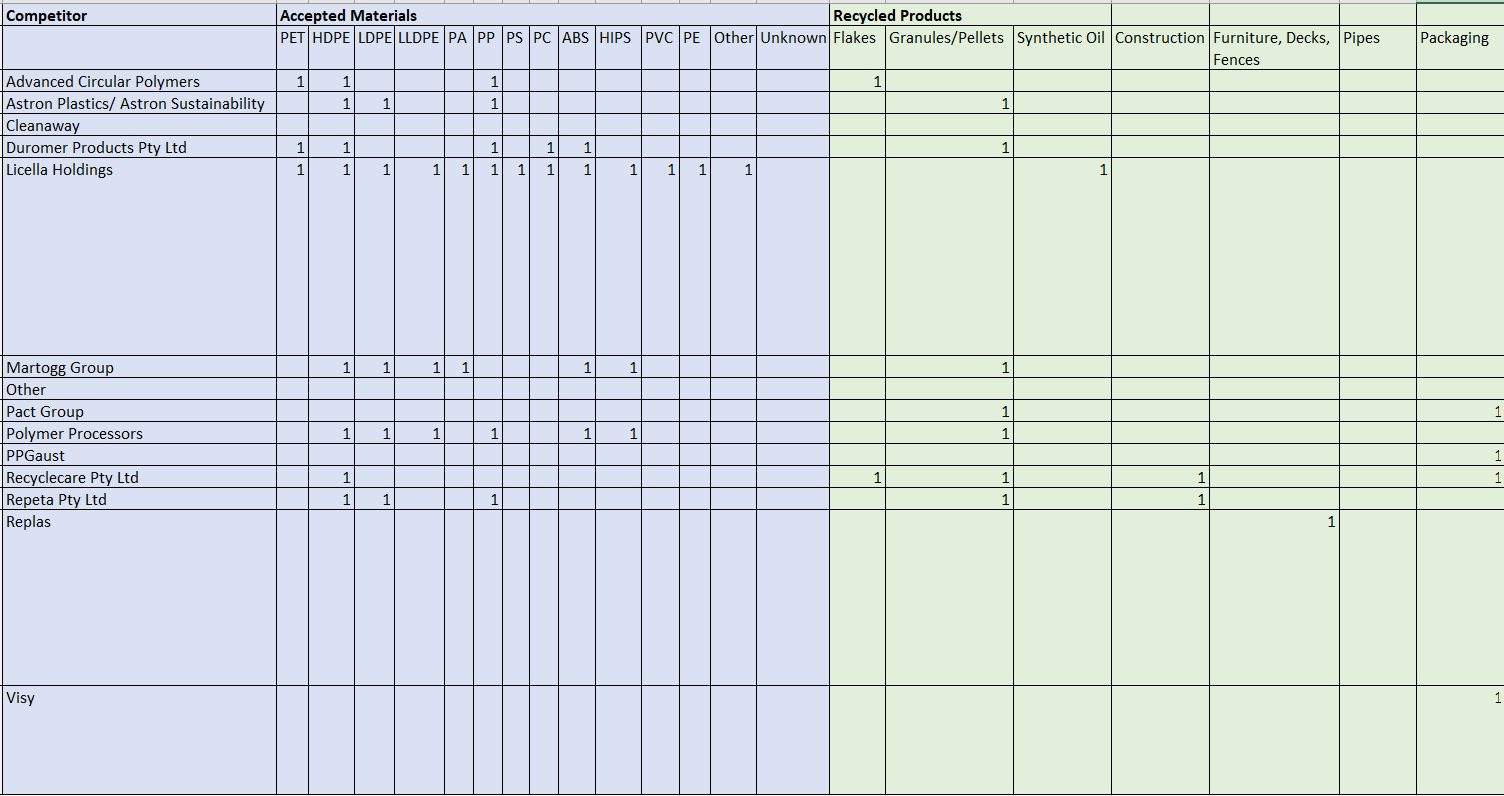
\includegraphics[width=\textwidth]{week7/accepted_products.png}
		\caption{Accepted Products}
		\label{fig:accepted_products}
	\end{figure}

\pagebreak

\section{Draft Report}
\label{app:draft}

	Draft report of target market work in Figure \ref{fig:draft}. Highlighted sections are my own words.

	\begin{figure}[h!]
		\centering
		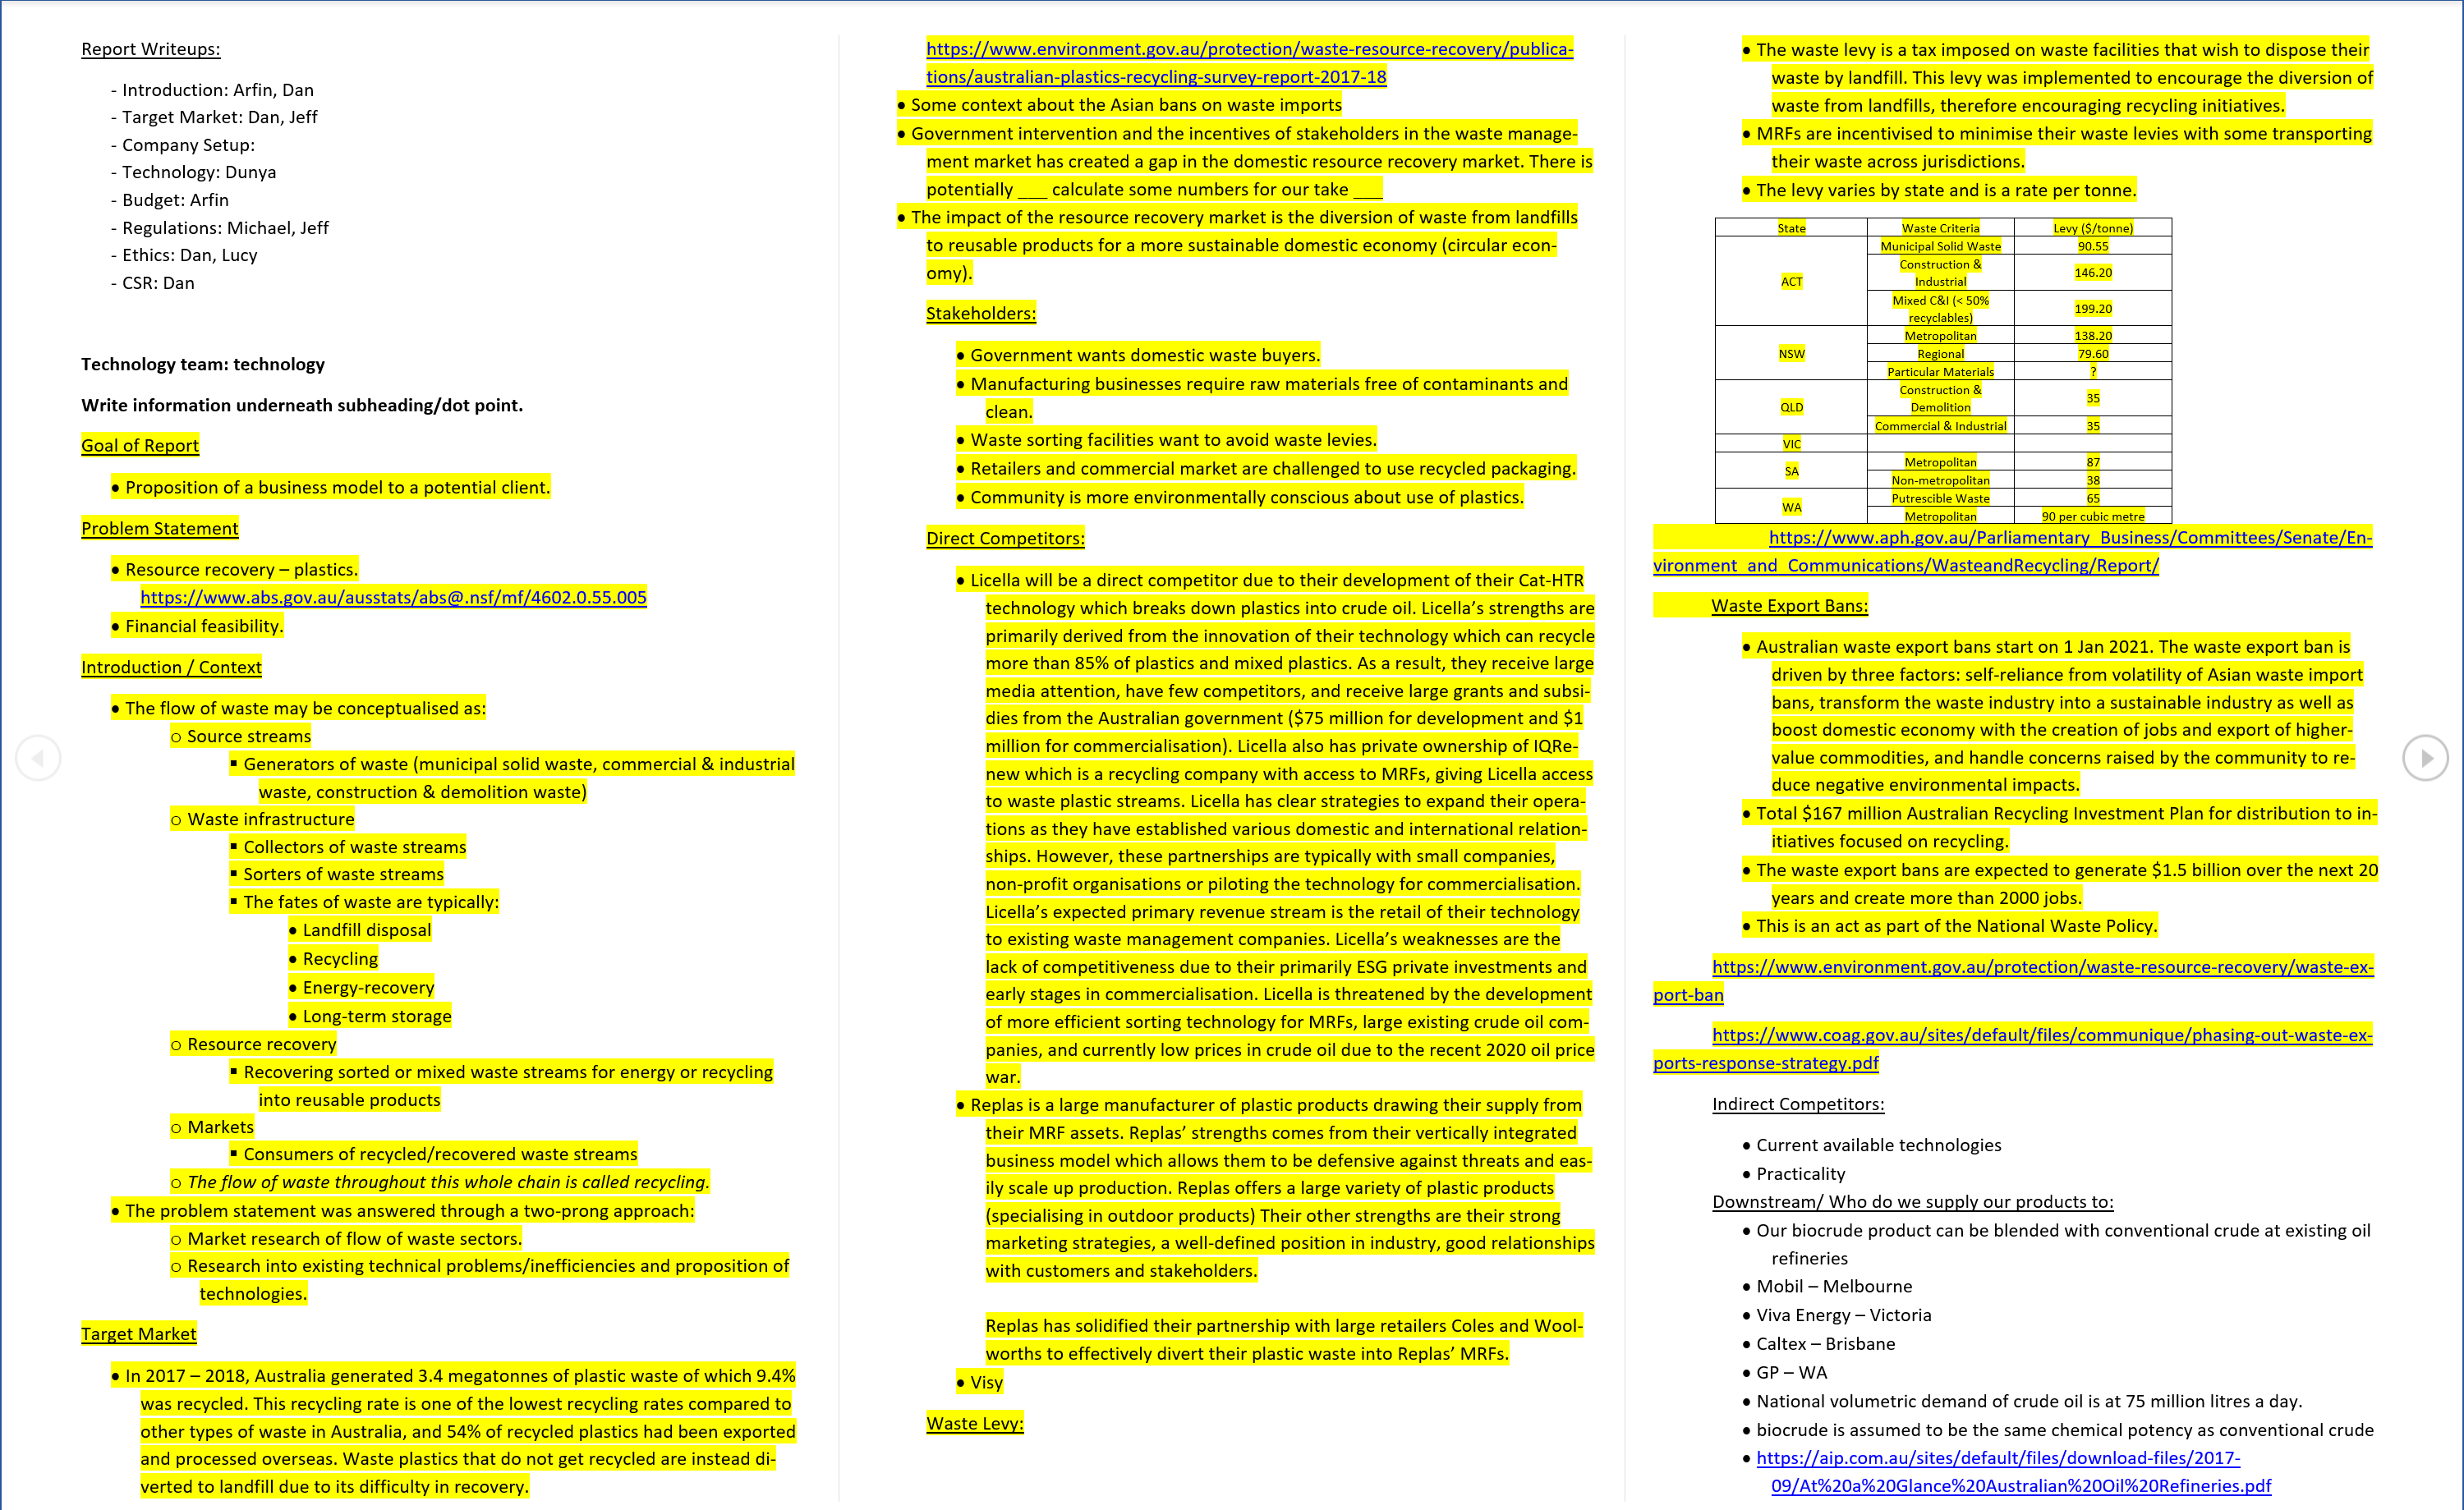
\includegraphics[width=\textwidth]{week8/draft_target_market.png}
		\caption{Draft Target Market}
		\label{fig:draft}
	\end{figure}

	Draft report of ethics in Figure \ref{fig:ethics}.

	\begin{figure}[h!]
		\centering
		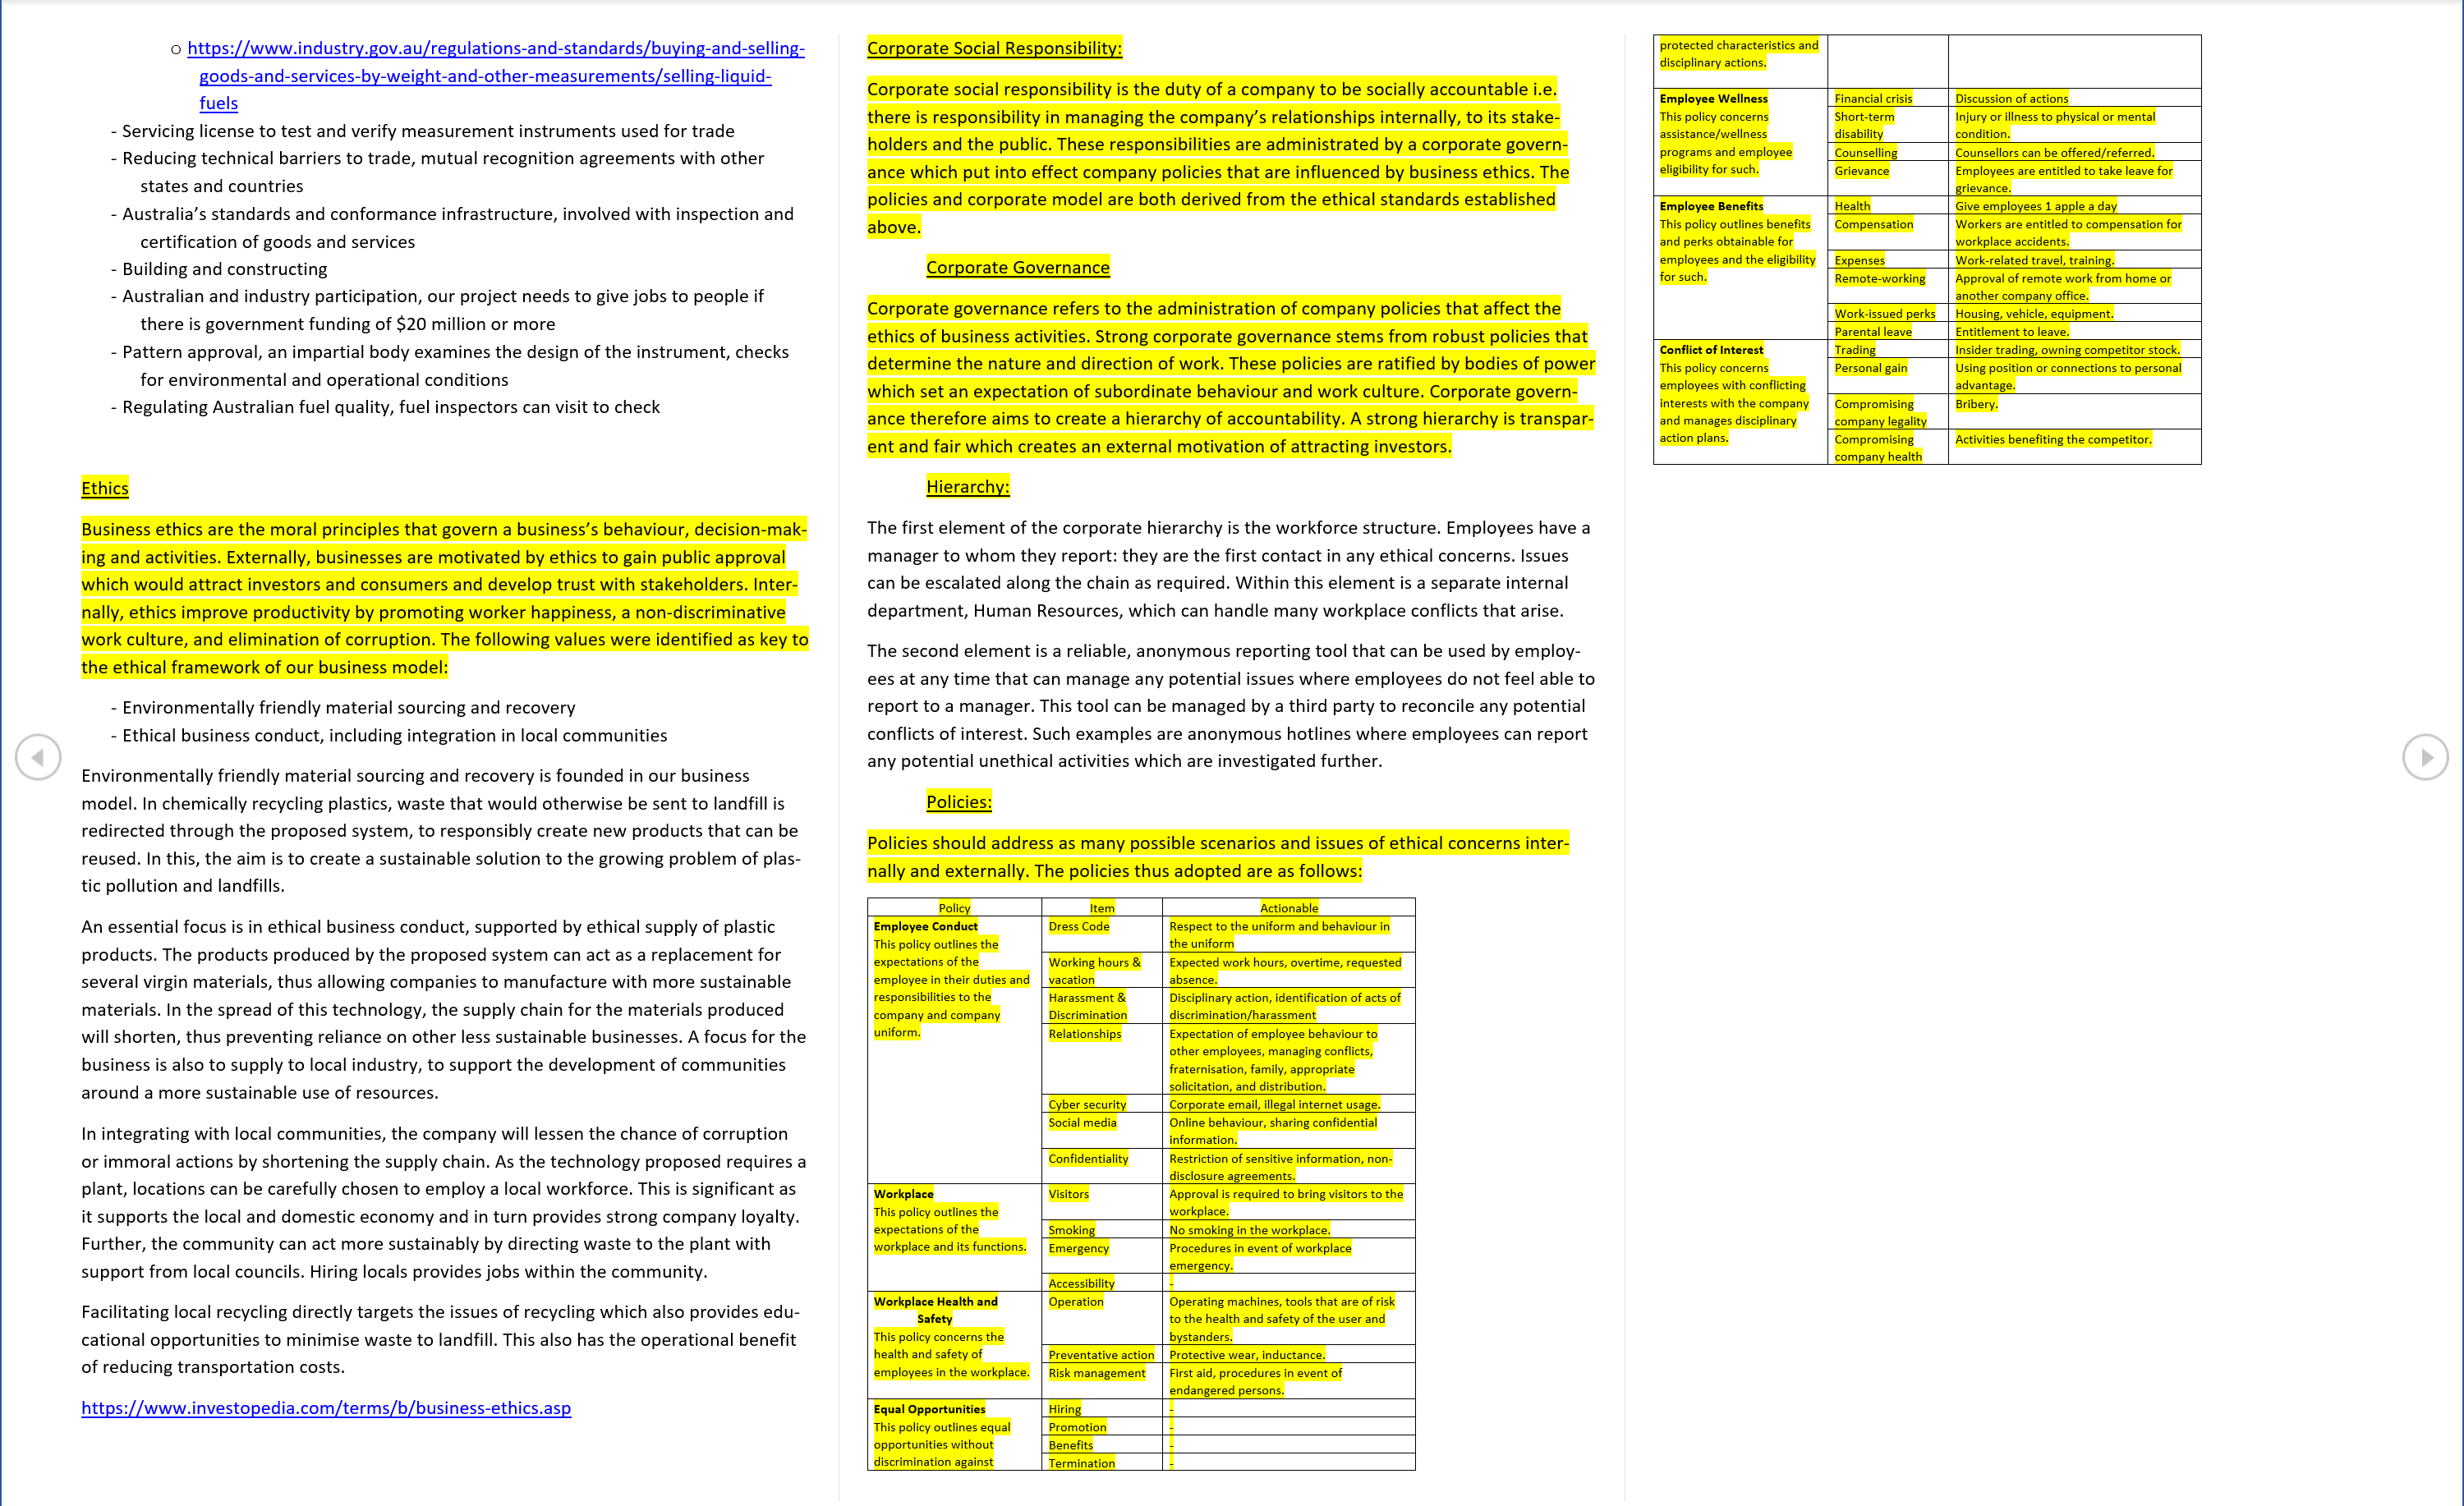
\includegraphics[width=\textwidth]{week9/draft_ethics_csr.png}
		\caption{Draft Ethics}
		\label{fig:ethics}
	\end{figure}

\pagebreak

\section{SWOT Analysis}
\label{app:swot}

	SWOT analysis of key and relevant players in domestic plastic resource recovery market in Figure \ref{fig:swot}.

	\begin{figure}[h!]
		\centering
		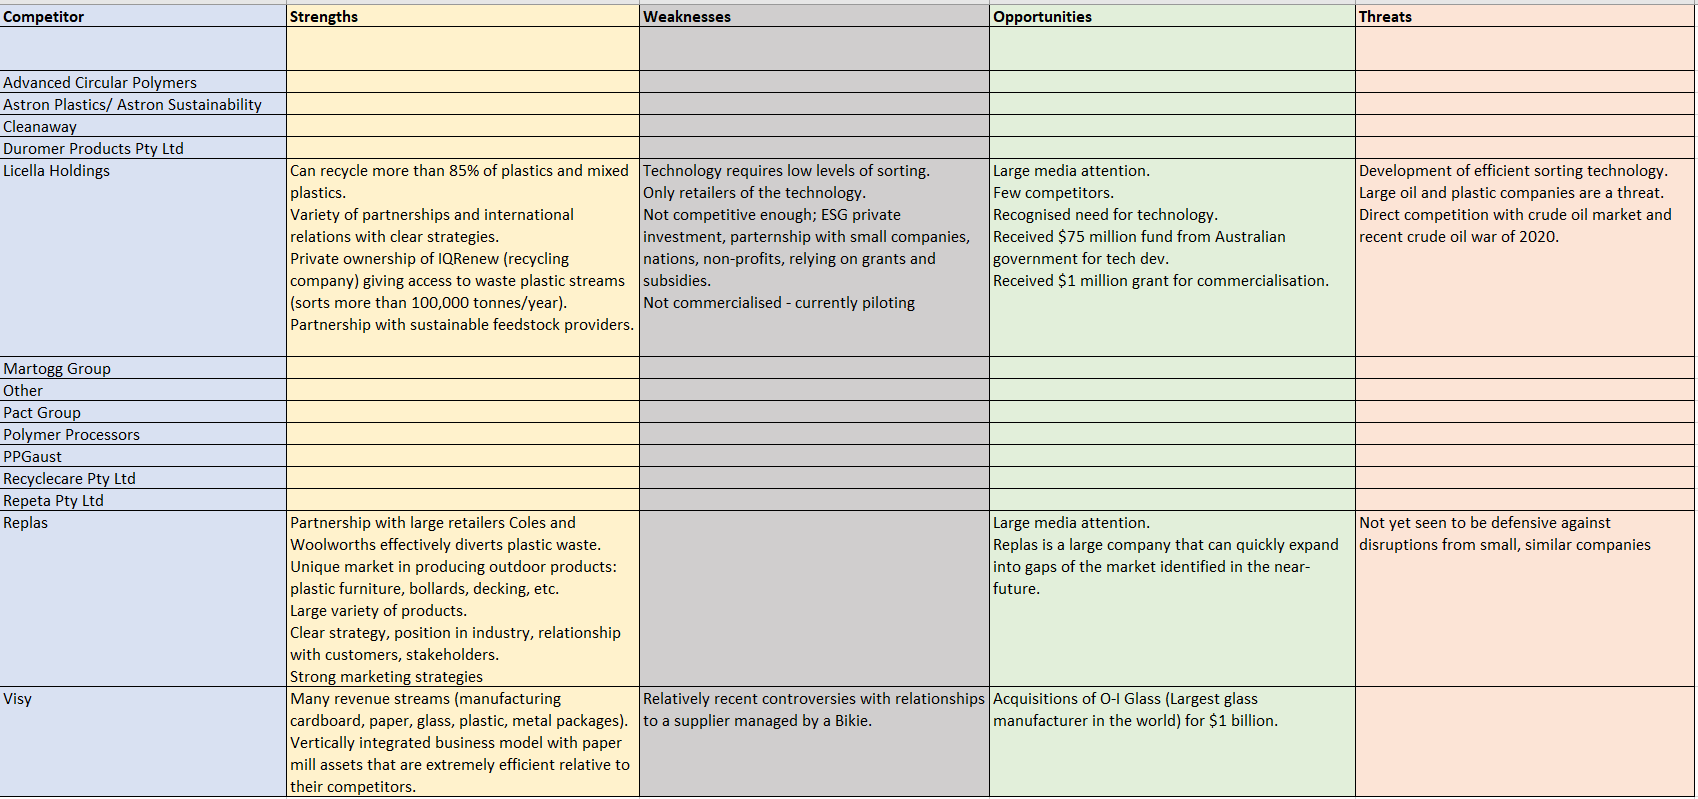
\includegraphics[width=\textwidth]{week8/swot_analysis.png}
		\caption{SWOT Analysis}
		\label{fig:swot}
	\end{figure}

\pagebreak

\section{Final Report}
\label{app:final}

	Text highlighted in yellow are my own words and in green are collaborated work or contributions to other work.

	Problem statement, introduction, target market research work in Figure \ref{fig:report1}.

	\begin{figure}[h!]
		\centering
		\fbox{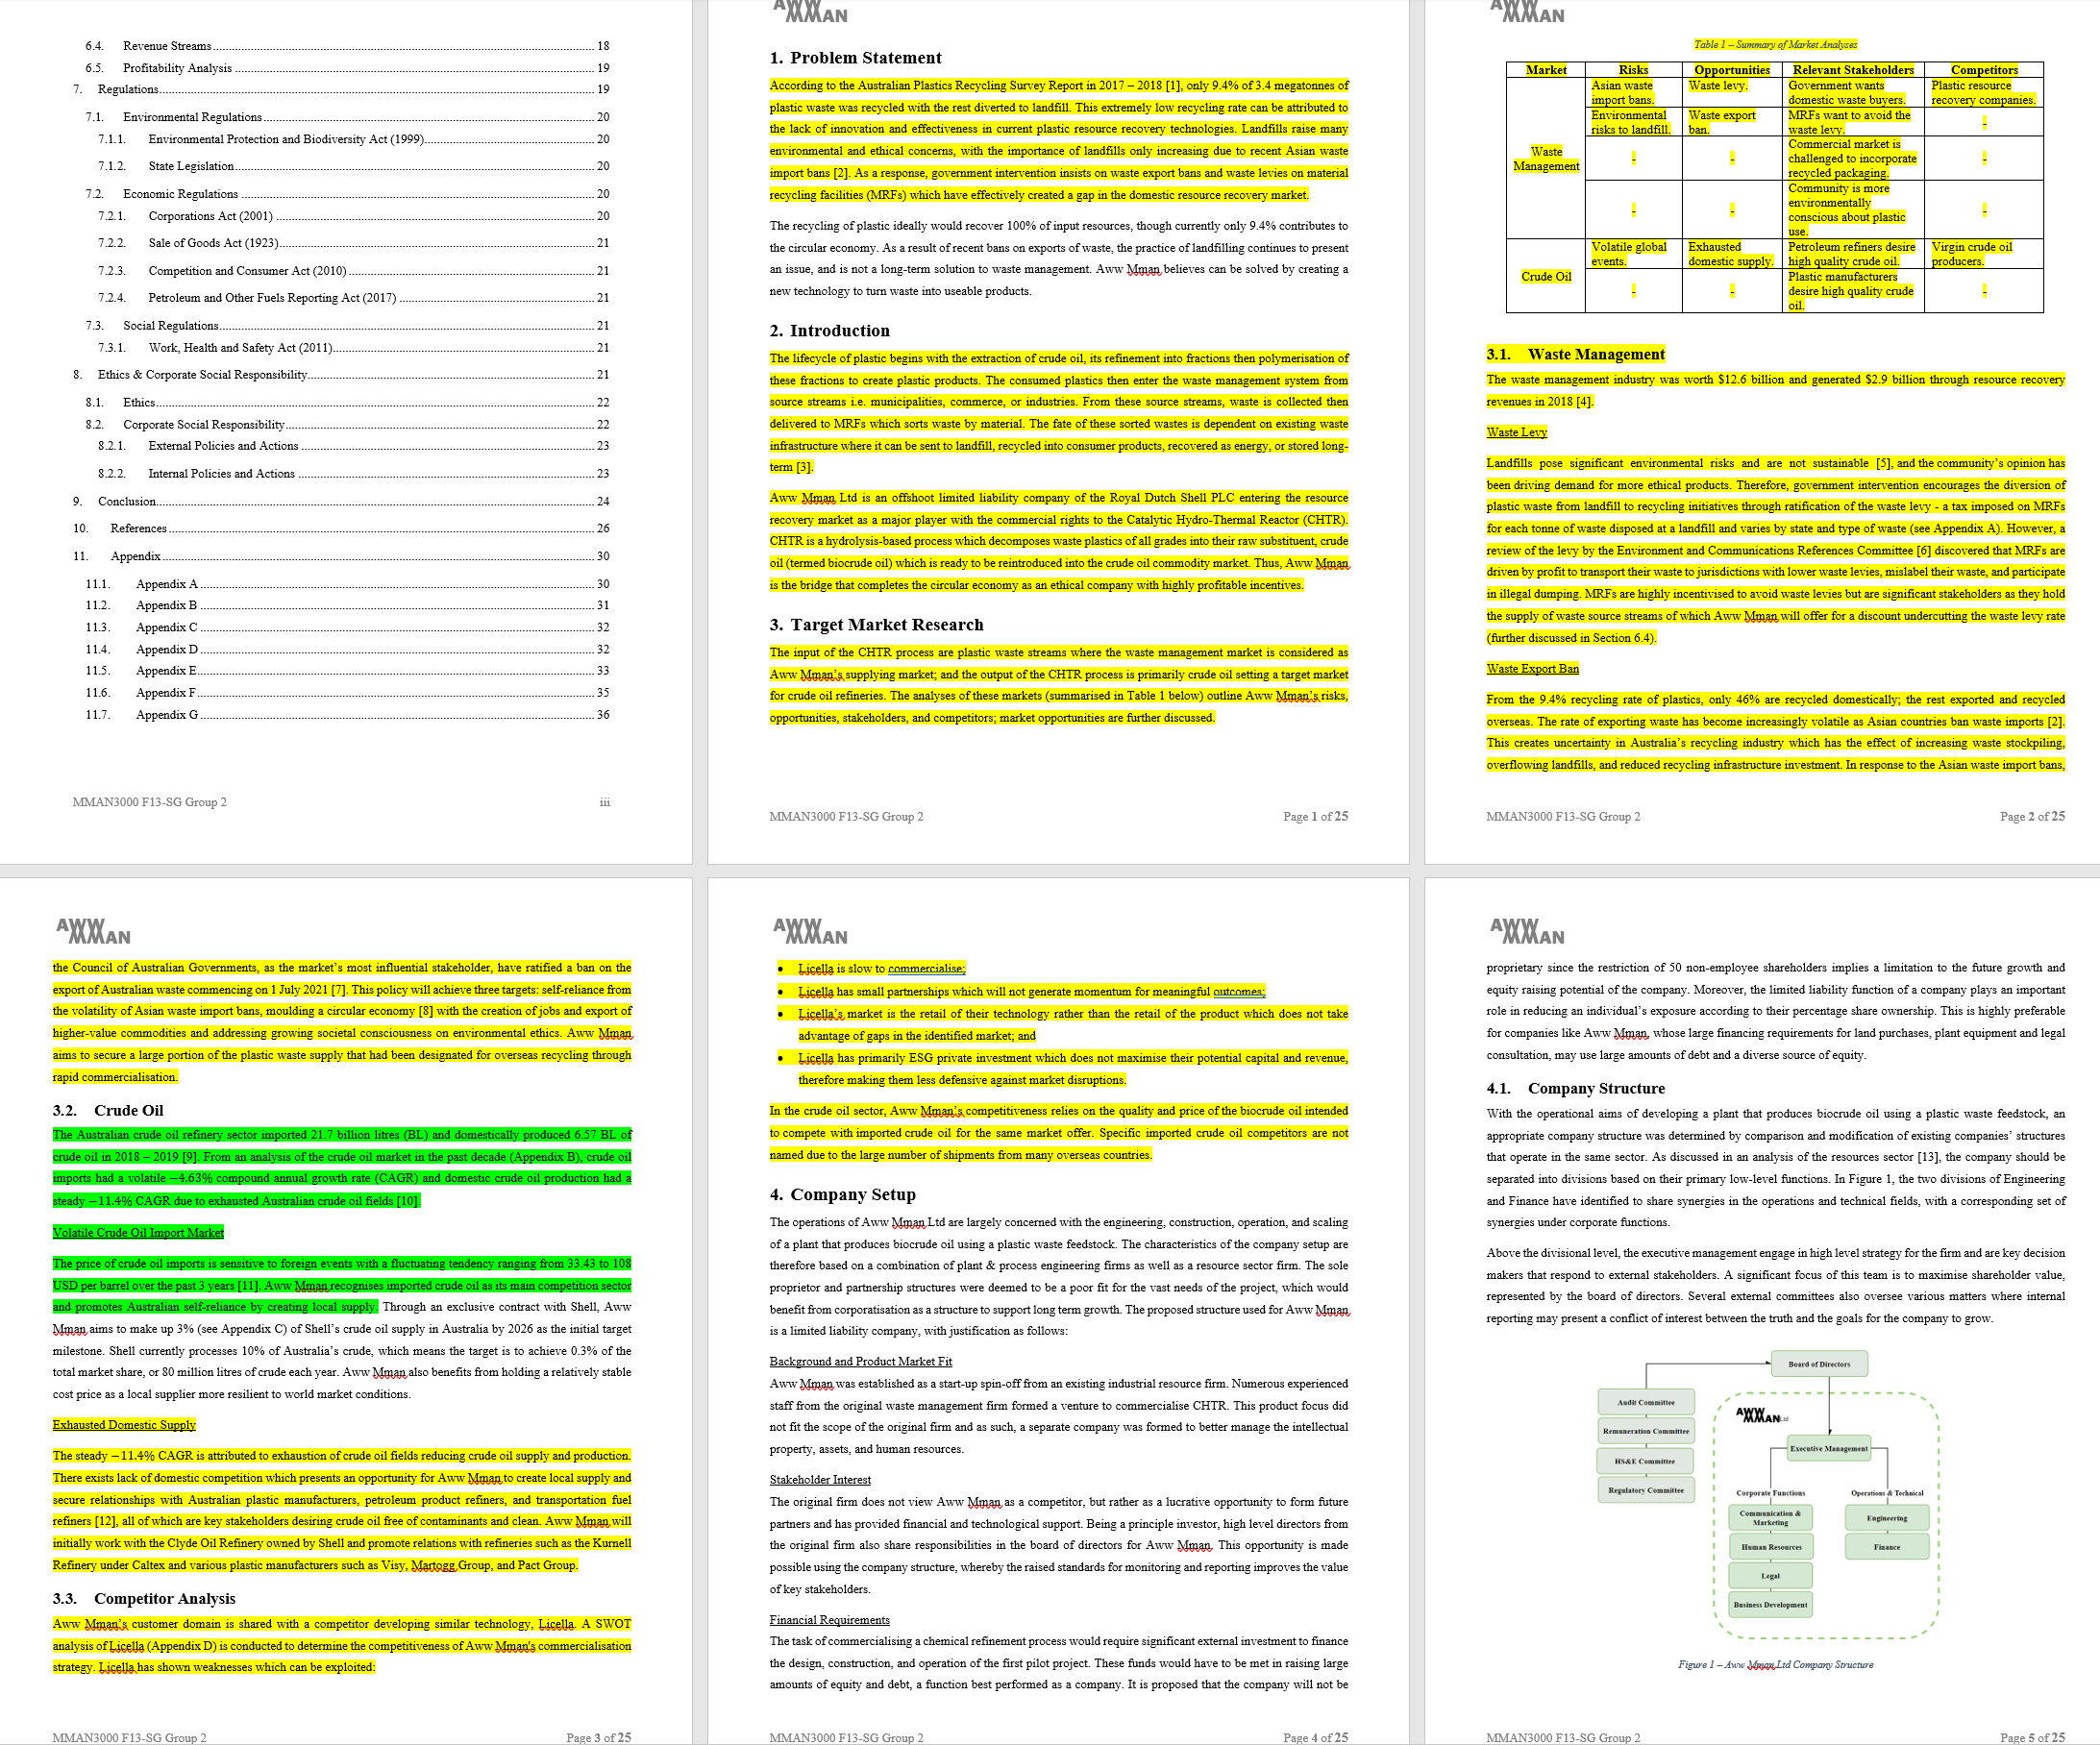
\includegraphics[width=0.98\textwidth]{week10/report1.png}}
		\caption{Problem Statement, Introduction, Target Market Report Work}
		\label{fig:report1}
	\end{figure}

	Corporate governance work in Figure \ref{fig:report2}.

	\begin{figure}[h!]
		\centering
		\fbox{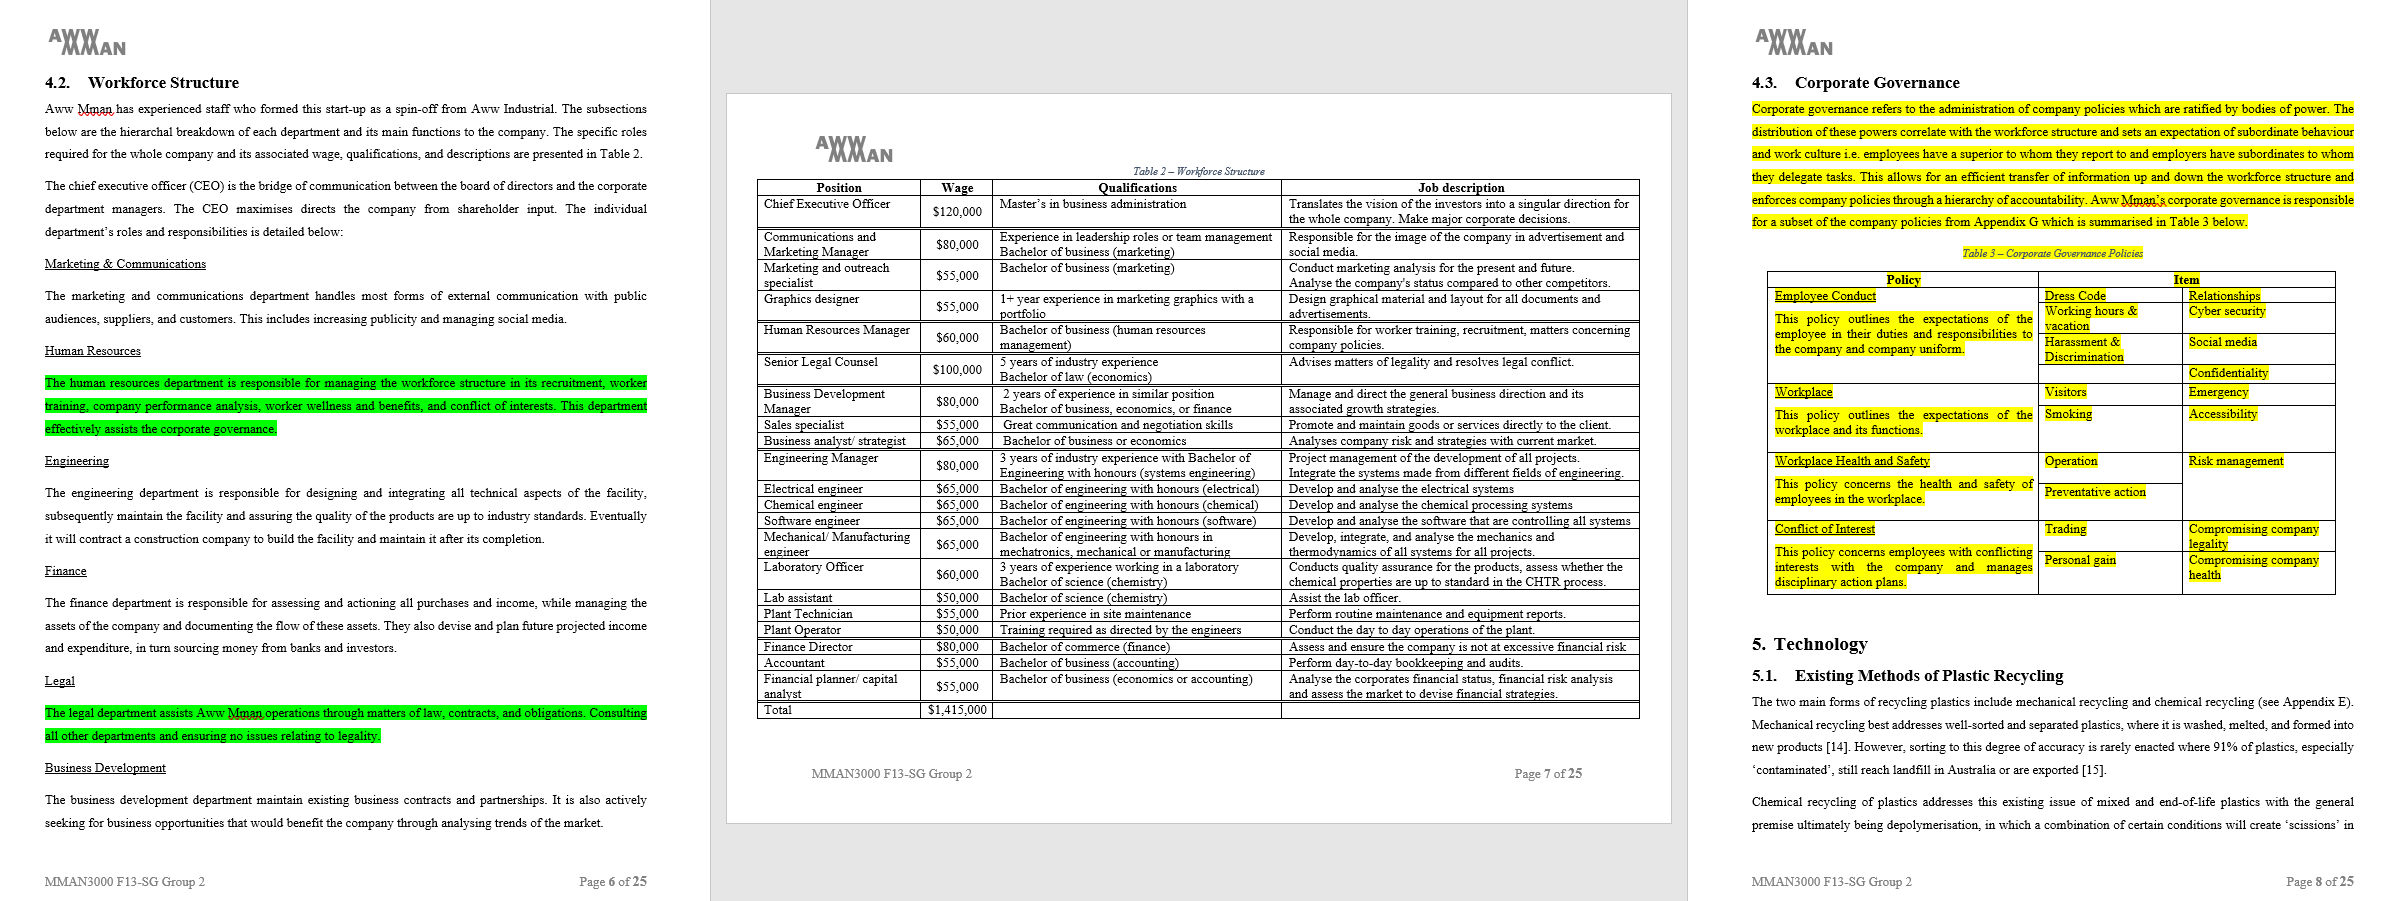
\includegraphics[width=0.98\textwidth]{week10/report2.png}}
		\caption{Corporate Governance Report Work}
		\label{fig:report2}
	\end{figure}

	Ethics and conclusion work in Figure \ref{fig:report3}.

	\begin{figure}[h!]
		\centering
		\fbox{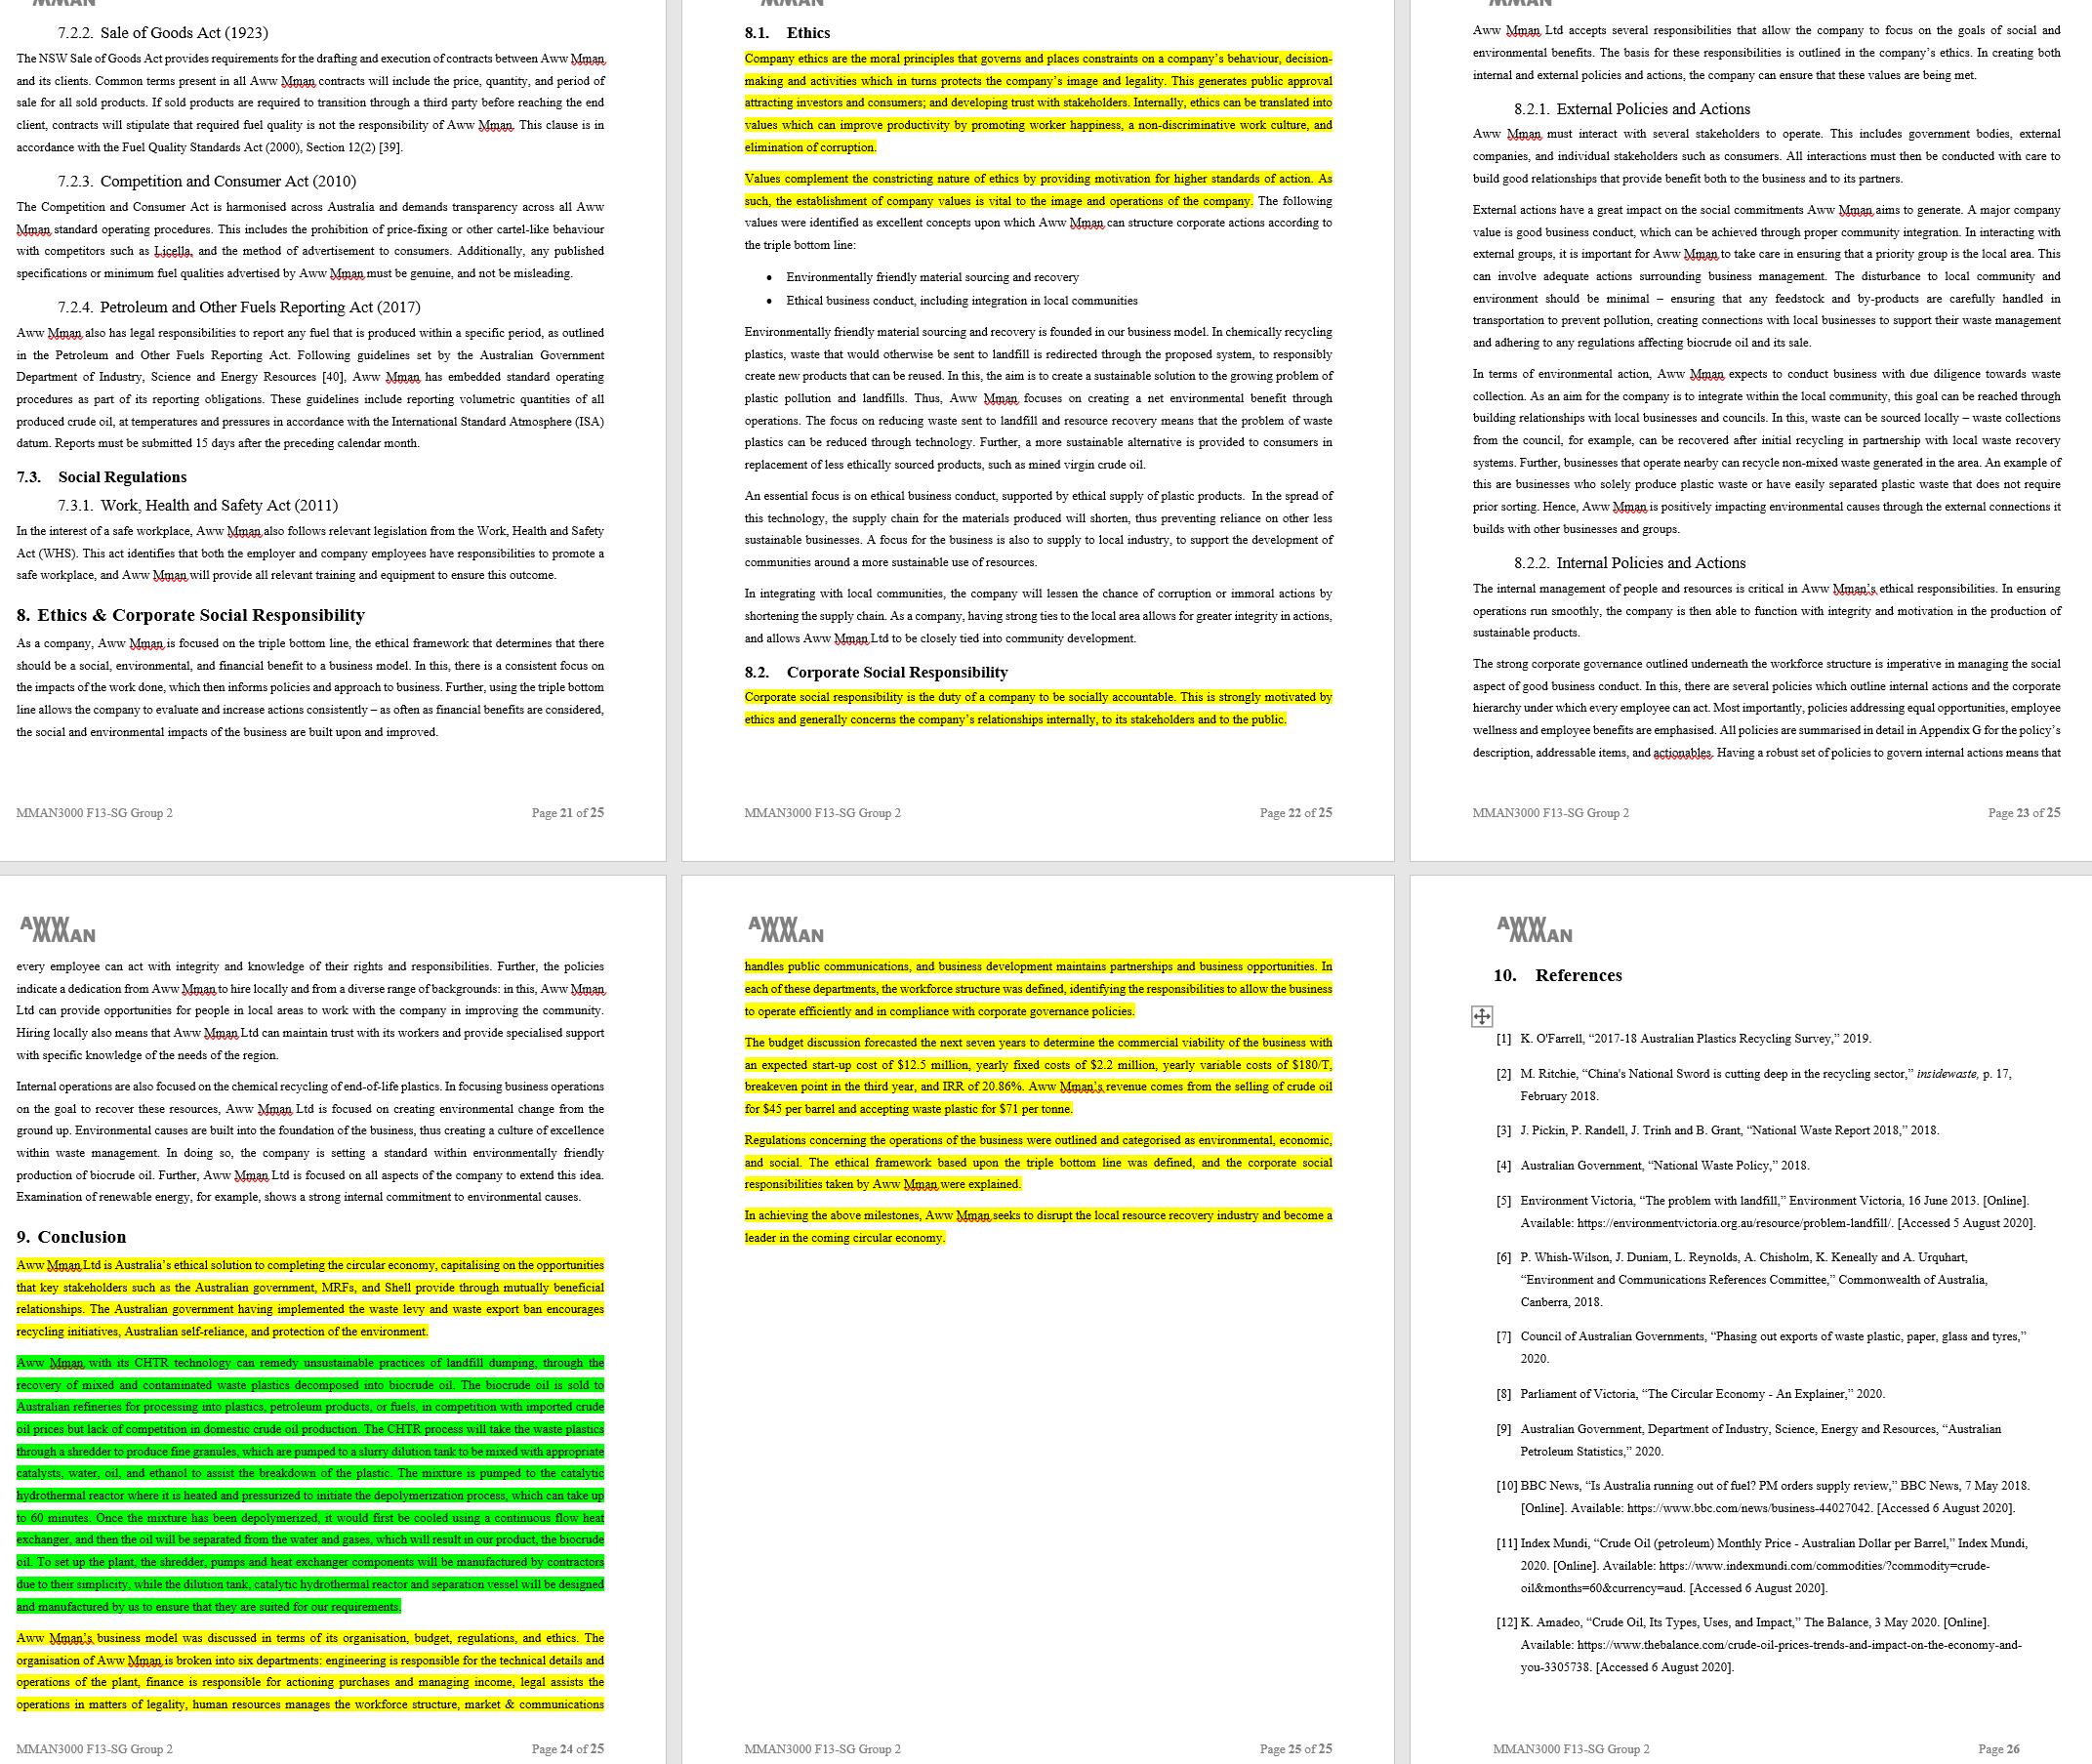
\includegraphics[width=0.98\textwidth]{week10/report3.png}}
		\caption{Ethics, Conclusion Report Work}
		\label{fig:report3}
	\end{figure}

	Appendix work in Figures \ref{fig:report4} and \ref{fig:report5}.

	\begin{figure}[h!]
		\centering
		\fbox{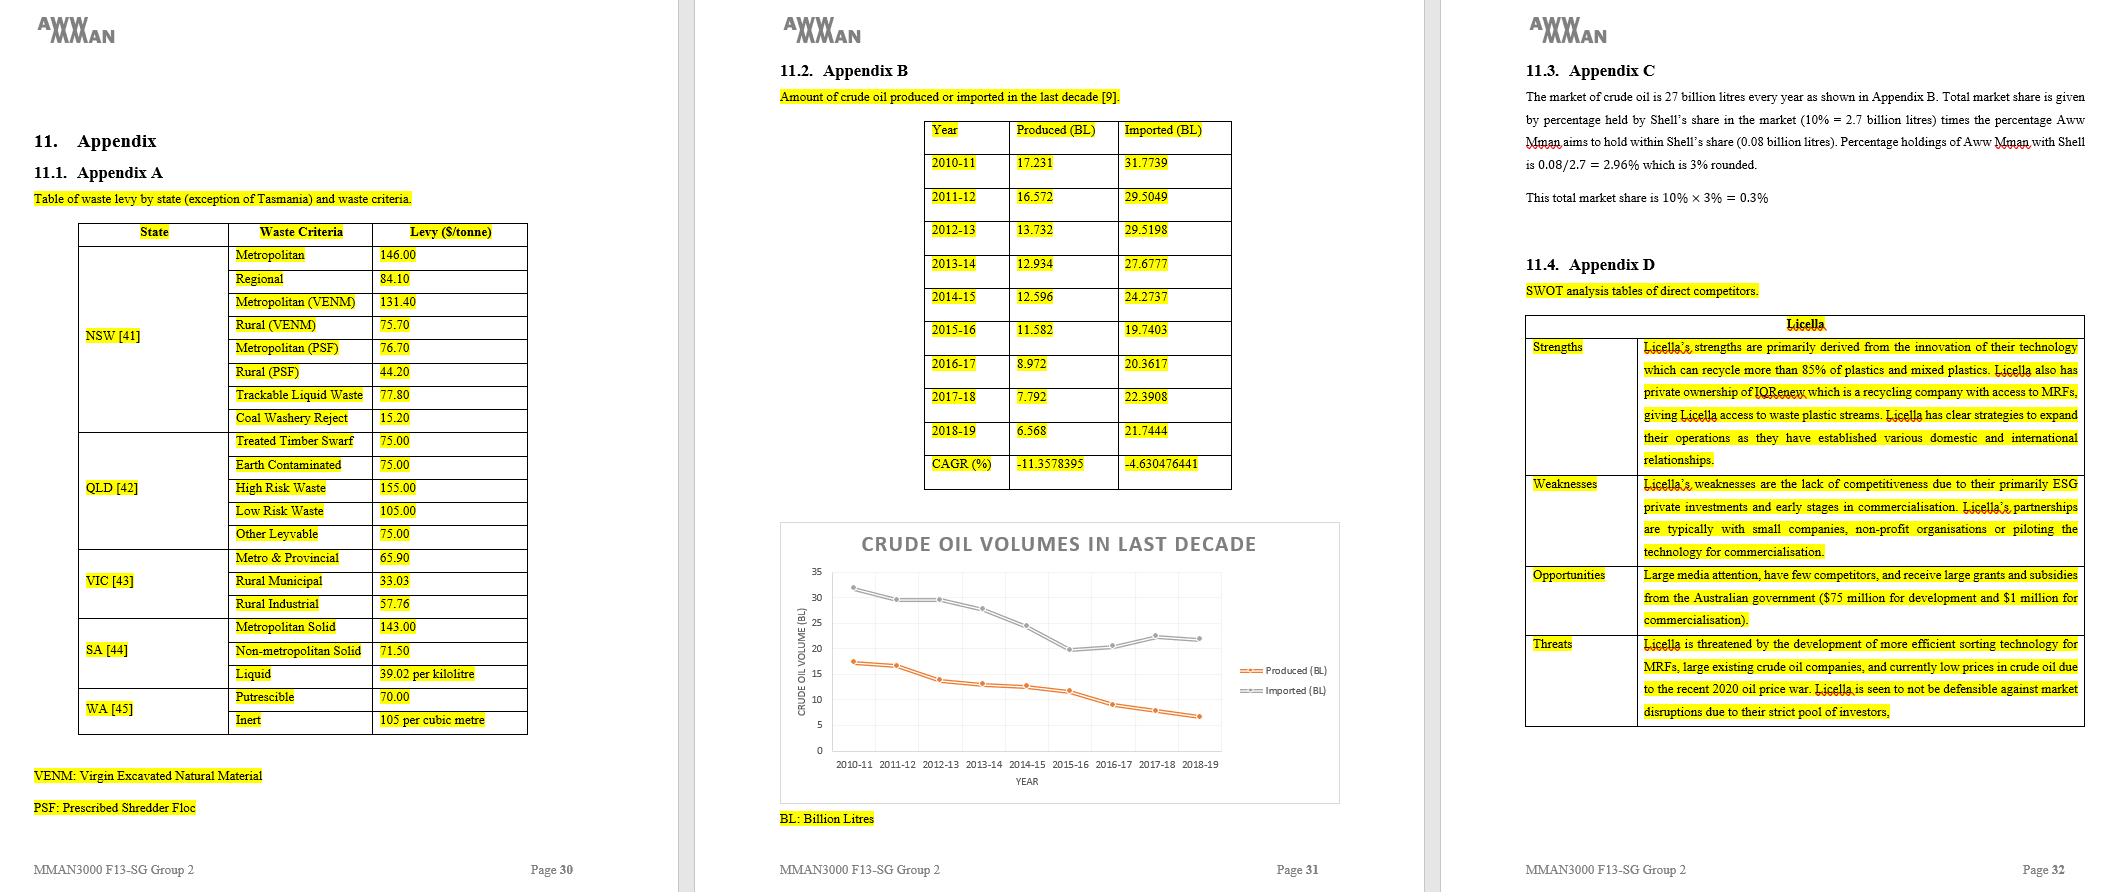
\includegraphics[width=0.98\textwidth]{week10/report4.png}}
		\caption{Appendix A, B, C Work}
		\label{fig:report4}
	\end{figure}

	\begin{figure}[h!]
		\centering
		\fbox{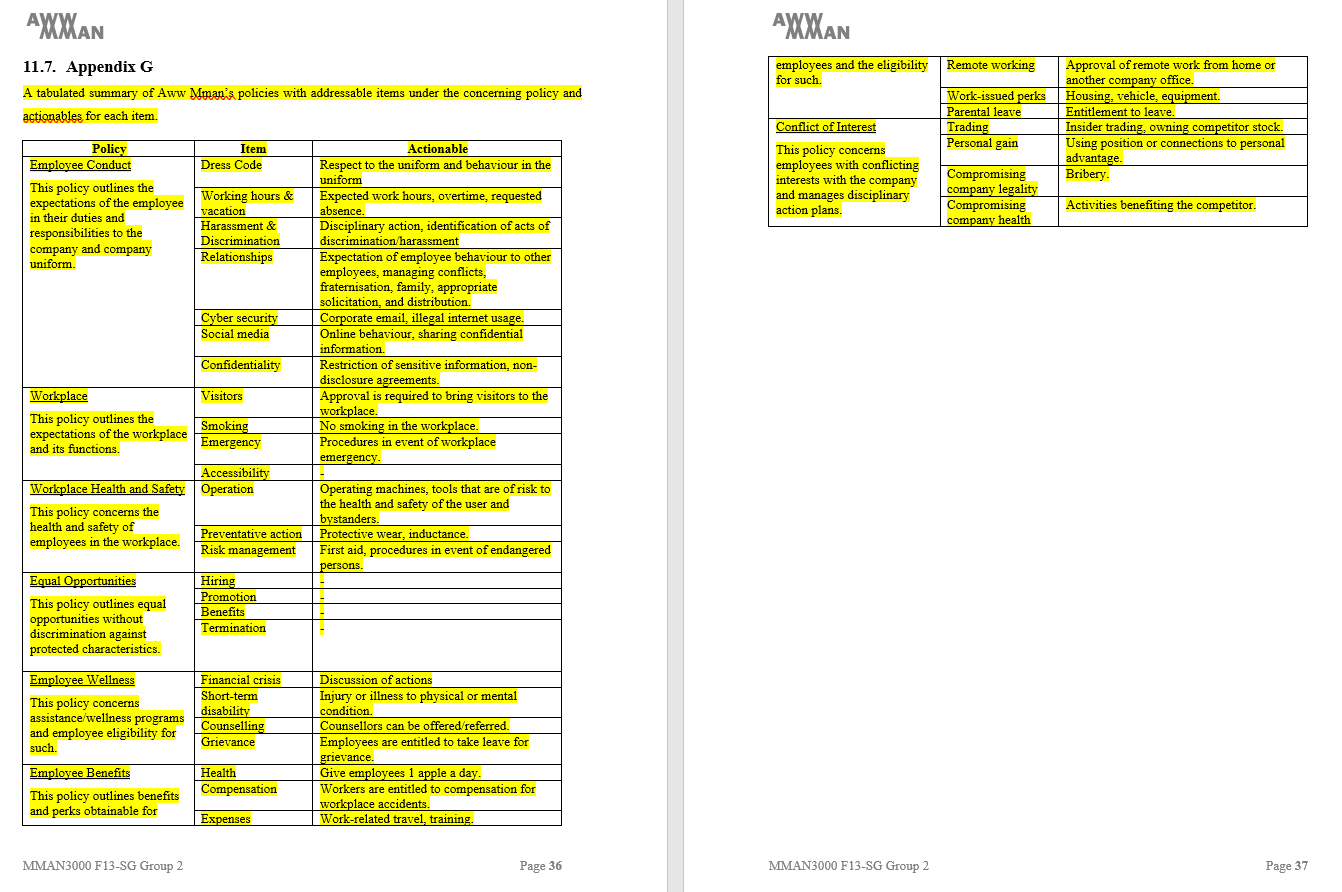
\includegraphics[width=0.98\textwidth]{week10/report5.png}}
		\caption{Appendix G Work}
		\label{fig:report5}
	\end{figure}

\pagebreak

\section{Marking Criteria}
\label{app:marking_criteria}

	Marking criteria used for self-evaluation and group evaluation (Table \ref{tab:criteria}). Each grade is worth one mark starting from zero, where grades are accumulated to give the total mark specified in the criterion.

	\begin{table}[h!]
		\scriptsize
		\centering
		\caption{Marking Criteria}
		\label{tab:criteria}
		\begin{tabular}{|C|D|D|D|D|D|D|}
			\hline
			\multirow{2}{*}{\textbf{Criterion}} & \multicolumn{6}{c|}{\textbf{Grade}} \\
			\cline{2-7}
			& 0 mark & 1 mark & 2 marks & 3 marks & 4 marks & 5 marks \\
			\hline
			Amount of Contribution (5 marks) & No effort. & Minimal effort. & Did not take up many tasks or completed few tasks. & Completed most tasks. & Completed all tasks. & Excellent initiative and completed all tasks. \\
			\hline
			Quality of Contribution (5 marks) & No effort. & Poor quality with no attention to detail. & Fair quality with some attention to detail. & Good quality with few mistakes. & Very good quality with few minor mistakes. & Excellent quality and attention to detail. \\
			\hline
			Chair Responsibility (3 marks) & Did not take responsibility. & Did not organise agendas and tried to take charge of meetings. & Organised agendas and tried to take charge of meetings. & Organised high-quality agendas and took charge of meetings. & - & - \\
			\hline
			Scribe Responsibility (2 marks) & Did not take responsibility. & Took poor-quality minutes. & Took high-quality minutes. & - & - & - \\
			\hline
			Morale (2 marks) & No enthusiasm or negative impressions. & Moderate enthusiasm. & High enthusiasm and encouragement. & - & - & - \\
			\hline
			Discussion (3 marks) & No effort or discouraged discussion. & Present but did not contribute to discussions. & Moderately participated to discussions & Actively participated to discussions. and opened dialogue. & - & - \\
			\hline
		\end{tabular}
	\end{table}

\end{appendices}

\end{document}